% Setup - do not change
\documentclass[11pt]{article}
\usepackage[top=0.9in, left=0.9in, bottom=0.9in, right=0.9in]{geometry} 
\usepackage{parskip}
\usepackage{multicol}
\usepackage[english]{babel}
\usepackage[utf8]{inputenc}
\usepackage{amsmath,amsthm,amssymb,graphicx,pdfpages,wrapfig,hyperref}
\usepackage[none]{hyphenat}
\usepackage{csquotes}
\usepackage{float}


\setlength\parindent{0pt}
%%%%%%%%%%%%%%%%%%%%%%%%%%%%%%%%%%%%%%%%%%%%%%%%%%%%%%%%%%%%%%%%%%%
% add other packages here if required

%% Bibliography are specified in this file. You can also choose inline bib style if you want to. But make sure your citation style is consistent (and proper)
% For more details on citation: https://library.unimelb.edu.au/recite
\usepackage[sorting = none]{biblatex}
\addbibresource{references.bib}

%%%%%%%%%%%%%%%%%%%%%%%%%%%%%%%%%%%%%%%%%%%%%%%%%%%%%%%%%%%%%%%%%%% the '%' symbol denotes comments

% Begin document creation
% DELETE THE \lipsum PLACEHOLDERS WHEN YOU BEGIN
\title{\textbf{How Does Viral Infection Affect Taxi Service Reliance?} \\ 
MAST30034 Assignment 1}
\author{
Xavier Travers \\
Student ID: 1178369 \\
%% Replace the link with your github repo
% 1. Remember to escape underscore in the link.
% 2. Remember to include the commit you want to submit in the link
\href{https://github.com/MAST30034-Applied-Data-Science/mast30034-project-1-DigitalData/tree/928e6d823c9c3953e2ae98ef8f2f9a46403a3a0c}{Github Repository}
}

\begin{document}
\maketitle

\section{Introduction}
% Link to a 30 min tutorial if you require revision: https://www.overleaf.com/learn/latex/Learn_LaTeX_in_30_minutes

Viruses are currently on everyone's mind due to the COVID-19 pandemic.
With the shift to working from home, lockdowns and fears of infection, 
it is natural to assume that many people-facing industries are no longer relied on as much.
% it is a natural assumption that many people-facing industries such as ride-hailing have suffered in demand.
To what extent is such an assumption true?
This report investigates possible correlations between a measure of reliance on taxi services, and virus case rates.
While most research is satisfied with measuring correlations with demand in the form of usage frequency, 
the focus for this report is placed on a measurement that is more reflective of reliance (or trust).

Specific to taxi services, a key measurement of reliance is average travel radius/distance.
This research is performed under the assumption that this measurement will correlate with the level of trust the average person places in a taxi service over alternatives.
For example, one may trust a taxi to travel further distances than the local tram.
Detailed throughout this report are steps taken to model average weekly trip distances against
the case rates of two prominent viruses: COVID-19 and Influenza.

\subsection{Timeline}
This report focuses on a single 24-month timeline starting in January 2020 and ending in December 2021.
Such a large timeline allows for aggregation on a per week basis to yield a large aggregate dataset.
It also includes a snippet of time before the COVID-19 pandemic for analysis.
Data from 2022 is not included to avoid any risk of using data that is so new that it is incomplete or hasn't been double-checked.
Data from before 2020 is not included to reduce code runtime when generating visualizations.
% Throughout this report, two timelines are used.
% \begin{itemize}
%     % \item \textbf{Timeline 2:} Starting in July 2018 and ending in June 2019.
%     % This 12-month timeline provides a window of time prior to the COVID-19 pandemic.
%     % It is used when data analysis focuses only on the effects of the Influenza virus 
%     % (since the effects of COVID-19 are likely confounding).
%     \item \textbf{Timeline 1:} Starting in July 2020 and ending in June 2021.
%     This 12-month timeline provides a window of time during the COVID-19 pandemic.
%     This timeline is used to construct linear models and generate other all other visualizations.
%     \item \textbf{Timeline 2:} Starting in July 2018 and ending in June 2021.
%     This 36-month timeline is used exclusively for time-series plots.
% \end{itemize}
\subsection{Datasets}
The New York City Taxi and Limousine Commission (TLC) provides a dataset of taxi service trips that captures information such as type of taxi, travel distance, general pick-up/drop-off locations/times and other trip data \cite{tlcdataset}. 
In this report, the focus is placed on New York's Yellow street hail taxis.
The subset of this data denoted by the timeline contains $64'913'648$ trips and $19$ features per trip before cleaning.
Also included from the same source is a mapping dataset for $265$ pick-up/drop-off locations and corresponding boroughs included in the TLC dataset \cite{tlcdataset}.

COVID-19 case rates have been recorded daily by the New York Department of Health and Mental Hygiene \cite{coviddataset}.
This dataset begins on the last day of February 2020, when the first official cases of COVID-19 were recorded in New York City. 
Each entry in this data set contains a date and several daily COVID-19 rates by borough (e.g. count of hospitalizations on the day in the Bronx).
Of specific interest throughout this report is the daily case count per borough.
This dataset contains $900$ rows and $67$ features per row before cleaning.

Influenza case rates are recorded on a weekly basis by the New York Department of Health \cite{fludataset}. 
Case rates in this dataset are aggregated by ``Morbidity and Mortality Weekly Report'' (MMWR) weeks, which are used by the United States Center for Diseas Control and Prevention (CDC) to number the weeks in each year\cite{mmwr}.
Each entry in this dataset is associated to an MMWR week, county (within the state of New York), type of Influenza (A, B or unspecified), and case count.
This dataset contains $77910$ rows and $9$ features per row before cleaning.

Since data is aggregated by borough, the population of each borough is accounted for.
For this purpose, the United States Census Bureau's yearly county population totals data is used \cite{populations2019, populations2020}.
This report specifically relies on the population estimates for the counties of New York State.
This data contains $16$ rows and $68$ columns per row (one column per county of New York State).

To provide a homogeneous time metric for aggregation, 
a dataset is generated that defines the MMWR weeks of the data within the selected timeline on a per borough basis.
This allows for easier grouping by borough with null values during weeks with no case rates or trips.
The MMWR weeks are generated according to the CDC's defined business rules \cite{mmwr}.
This generated MMWR week dataset contains $3675$ rows and $11$ features per row.

All of these datasets provide coverage over the chosen timeline of analysis, 
allowing for the generation of meaningful models.
For geospatial visualizations, 
the City of New York's Department of City Planning provides a dataset containing borough outlines \cite{boroughdataset}.
This contains the geometry of each borough as well as their names.
This dataset contains $5$ rows and $5$ features per row.


% \LaTeX{} Have many caveats, you should search stack overflow for latex tips whenever you feel something looks bad, for instance:
% When `` quoting '', should be used instead of ". For example, ``test'' vs "test".

% % use \textbf{} for bold text and \textit{} for italic. 
% % \texttt{} creates code blocks akin to `code ticks` in markdown
% \textbf{Please refer to the spec, the word count and page count is strict.} Feel free to change the section headings (and we recommend you do).

% Always remember to cite materials that does not belong to you. For instance, you should cite the sensor datasets \cite{2022sensorreading, 2022sensorlocation}.
% % Example here used biblatex to manage citations: https://www.overleaf.com/learn/latex/Bibliography_management_with_biblatex , You are free to choose your own way for managing references if biblatex seems too hard.

% \lipsum[7]

% You can have \section{}, \subsection{}, and \subsubsection{}
\section{Method}

\subsection{Preprocessing}

The datasets require the removal of several entries, 
and steps taken to generate aggregate data for proper analysis.
The flu dataset contains detail only on a weekly basis, 
while the other datasets contain daily data. 
Thus, the most granular time unit by which the data can be analysed is the MMWR week.
This potential weakness in the analysis is discussed in this section as well.

\subsubsection{Cleaning}

There are several processes used to remove outliers and unwanted data.
Noted are the steps taken to ensure that aggregation by borough and MMWR week is achievable with the TLC, COVID-19 and Influenza datasets.
Imputation is performed on the virus data where no cases were reported for a week or data.
The case counts for these non-included rows are assumed to be $0$, 
since the datasets are unlikely to contain missing data due to their importance to the CDC.

\textbf{Borough vs. County:} Each of the 5 boroughs of New York City correspond to a county recognized by New York State \cite{countytoborough}.
Some datasets contain counties, while others define statistics per borough. The boroughs with corresponding counties of different names are: 
Manhattan, also called New York County; 
Staten Island, also called Richmond County;
and Brooklyn, also called Kings County \cite{countytoborough}.

\textbf{TLC Dataset:}
% \begin{multicols}{2}
    \begin{enumerate}
        \item Derive trip duration (in hours) and trip speed (in MPH) columns. 
        Filter out illegal (and likely incorrect) trip entries with a speed greater than 65 MPH, 
        as per New York State law \cite{laws}.
        \item Discard all columns except the pick-up time, trip distance, and pick-up location ID.
        \item For each entry, find the associated pick-up borough. 
        Discard all rows where pick-up is not within the 5 boroughs.
        \item Discard rows with null values in the above columns or where there is negative distance.
        \item Derive the MMWR week associated to each trip entry, as well as the year and month that the majority of the week participates in.
        Discard all rows where the MMWR week is not within Timeline 1.
    \end{enumerate}
% \end{multicols}
Since only the trip distance is of concern in this report,
filtering on other columns is not deemed necessary as long as the entries for trip distance and pick-up borough are consistent and valid.

\textbf{COVID-19 and Influenza Datasets:}
These datasets are very simple, and therefore require very little preprocessing.
First, the case counts per day (or per week, for the Influenza dataset) per borough are extracted. 
Then, the MMWR week associated to each entry, as well as the year and month that the majority of the week participates in are derived (where necessary).
Finally, all rows where the MMWR week is not within Timeline 1 are discarded.
For the Influenza dataset, 
counties are converted to their associated borough names for homogeneity of data.

\subsubsection{Aggregation}

\textbf{TLC Dataset:}
This dataset is aggregates by MMWR week and pick-up borough.
This allows for a granular look at potential pattern differences between the reliance measures grouped by pick-up locations.
The aggregated set is then joined by MMWR year and borough to the corresponding population estimate.
For the groupings described above, the number of trips,
the average trip distance and passenger count is calculated.
This aggregation over Timeline 1 results in approximately $52$ rows per borough.

This report only performs grouping by pick-up location,
allowing models to reflect a potential taxi customer's perspective on their immediate surroundings before taking a trip.
However, exploration of differences between grouping by pick-up or drop-off location on the results of models 
is a recommended extension to this research.

\textbf{COVID-19 and Influenza Datasets:}
Similarly to the above, the datasets are grouped by MMWR week information and borough where necessary.
This grouping is joined by MMWR year and borough with the corresponding borough's population estimates in a given year.
For each grouping, the weekly case rate per 100'000 people in the borough is calculated.

\textbf{Aggregation Averages:}
Since aggregation is performed on a mass scale, there is the risk of losing a lot of information present in the granularity of per-trip or per-day datasets.
However, aggregating on a mass scale is beneficial in that the averages calculated (for distance and passenger count)
a less prone to variability. As described by the Central Limit Theorem, as sample size $n$ increases for a sample mean $\bar{X}$, 
$\text{var}(\bar{X}) \propto \frac{1}{n}$. Therefore, since there over 150 million trips contained within Timeline 1, the sample size per week per borough is in the hundreds of thousands trips (assuming an even distribution of trips),
minimizing the variance of the sample means used.

\pagebreak
\subsection{Analysis and Modelling}

This section of the report highlights the analysis performed on the aggregated data
and describes the models generated for passenger counts and trip distances.

\subsubsection{Preliminary Analysis}

\textbf{Time-Series Analysis:}
Shown in Figure~\ref{fig:ts} is the change in average trip distance over time. Interestingly, 
while most boroughs (pick-up or drop-off) experience a slump in average trip distance following the "COVID dip", 
Staten Island appears to recover from the effects, and even increase in average trip distance
during the COVID-19 pandemic.

% This uptick in travel distance is likely caused by reduced usage of the Staten Island ferry and the reduced schedule during the pandemic \cite{dot2020}.
% If this is the case, then Figure~\ref{fig:ts} suggests that people travelling to and from Staten Island rely on taxis to be safer and ontime over the ferry service.
% The trip distances between boroughs are generally not very homoegeneous. 
% A likely reason for this heterogeneity is the difference in commutes to work, since
% many jobs are likely located in Manhattan.

\begin{multicols}{2}
    This uptick in travel distance is likely caused by reduced usage of the Staten Island ferry and the reduced schedule during the pandemic \cite{dot2020}.
    If this is the case, then Figure~\ref{fig:ts} suggests that people travelling to and from Staten Island rely on taxis to be safer and ontime over the ferry service.
    The trip distances between boroughs are generally not very homoegeneous. 
    A likely reason for this heterogeneity is the difference in commutes to work, since
    many jobs are likely located in Manhattan.
    The greatest instability in trip distances appears in trips going from Staten Island,
    while travel from other boroughs appears more stable and similar week-on-week. 
    % \begin{figure}[H]

    %     \centering
    
    %     % change the scale multiplier to make the figures smaller or larger
    %     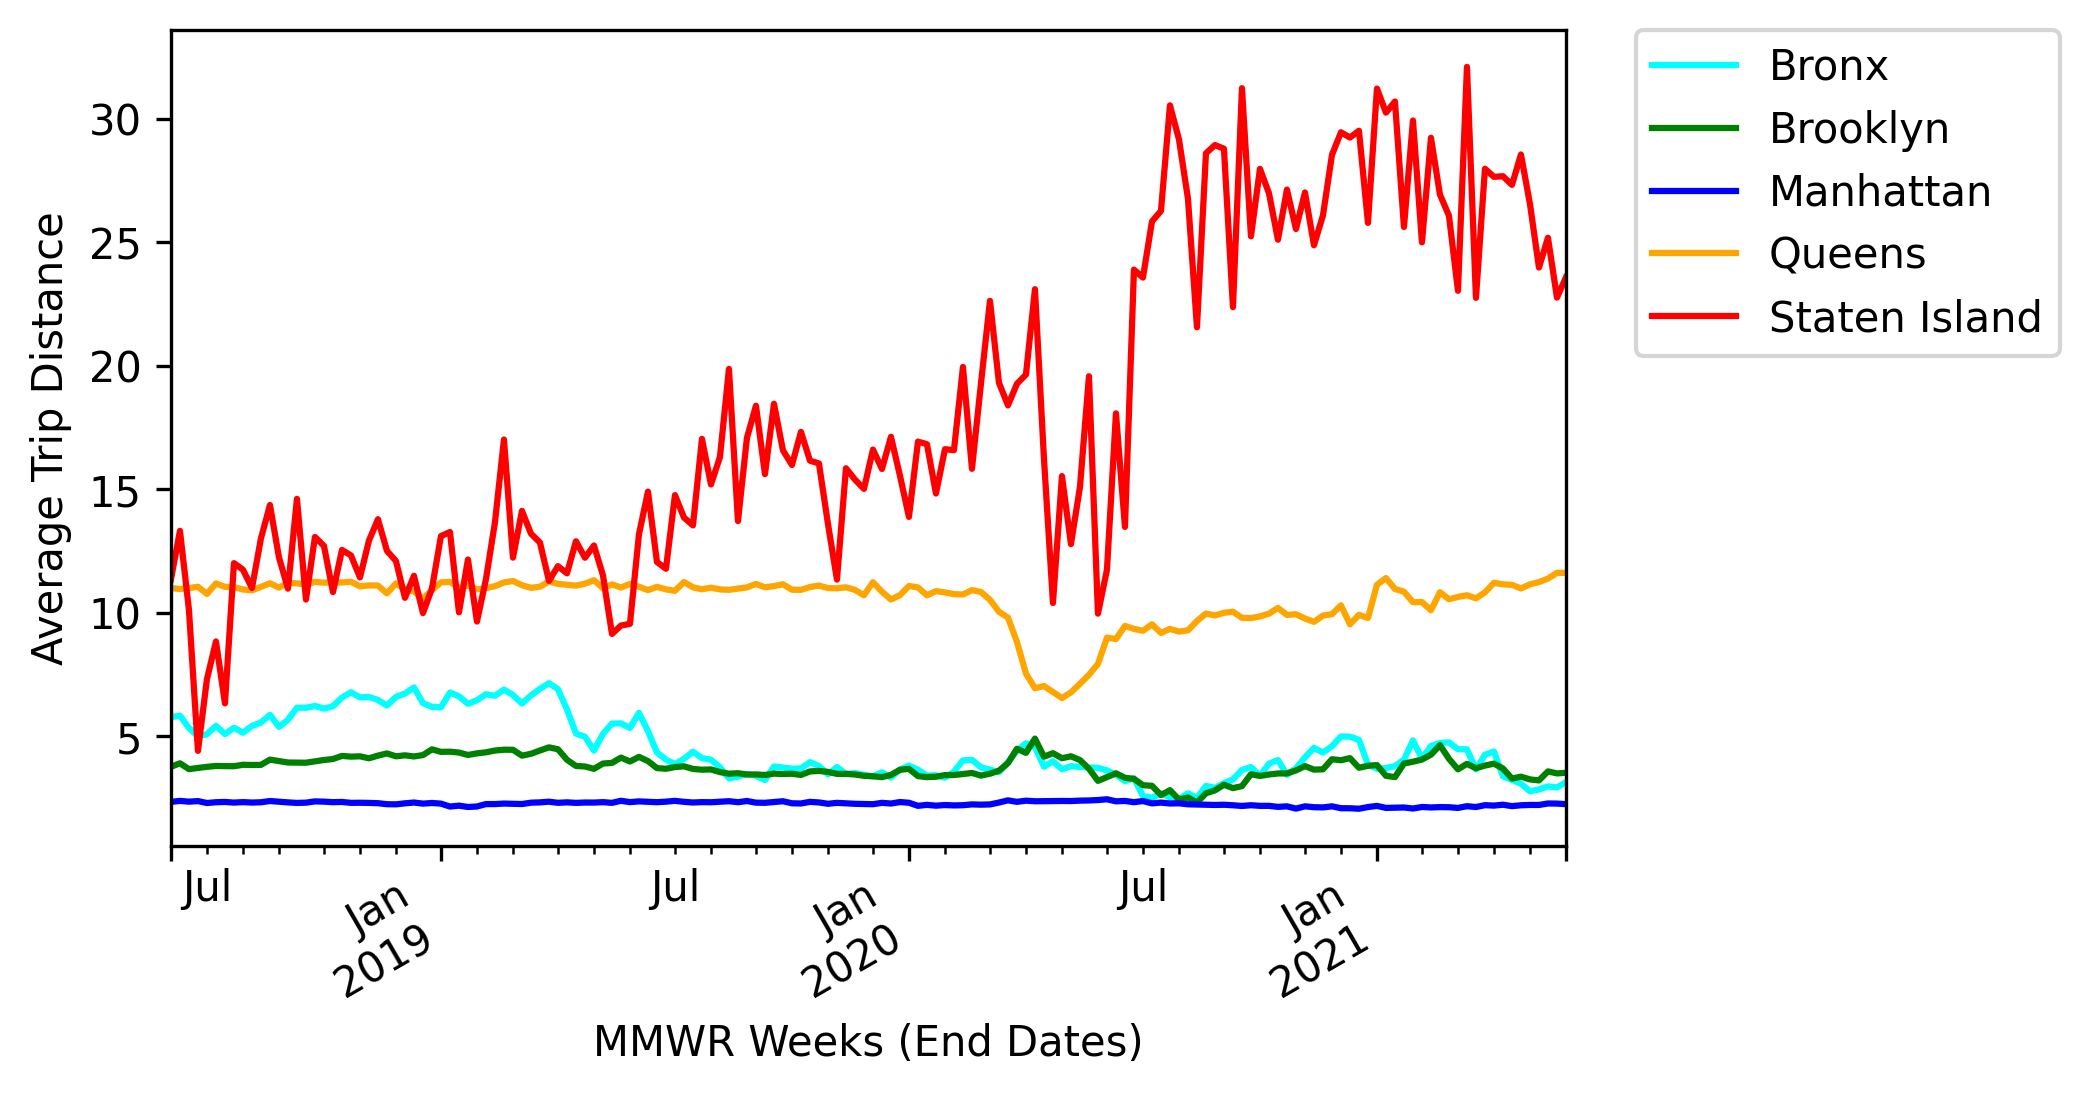
\includegraphics[width=0.54\textwidth]{../plots/time-series-Average Trip Distance-vs-MMWR Weeks (End Dates)-by-pu_borough.png}
    %     \caption{How average trip distances per week per pick-up borough vary over time.} % refer to this image as (Figure 1)
    
    %     % 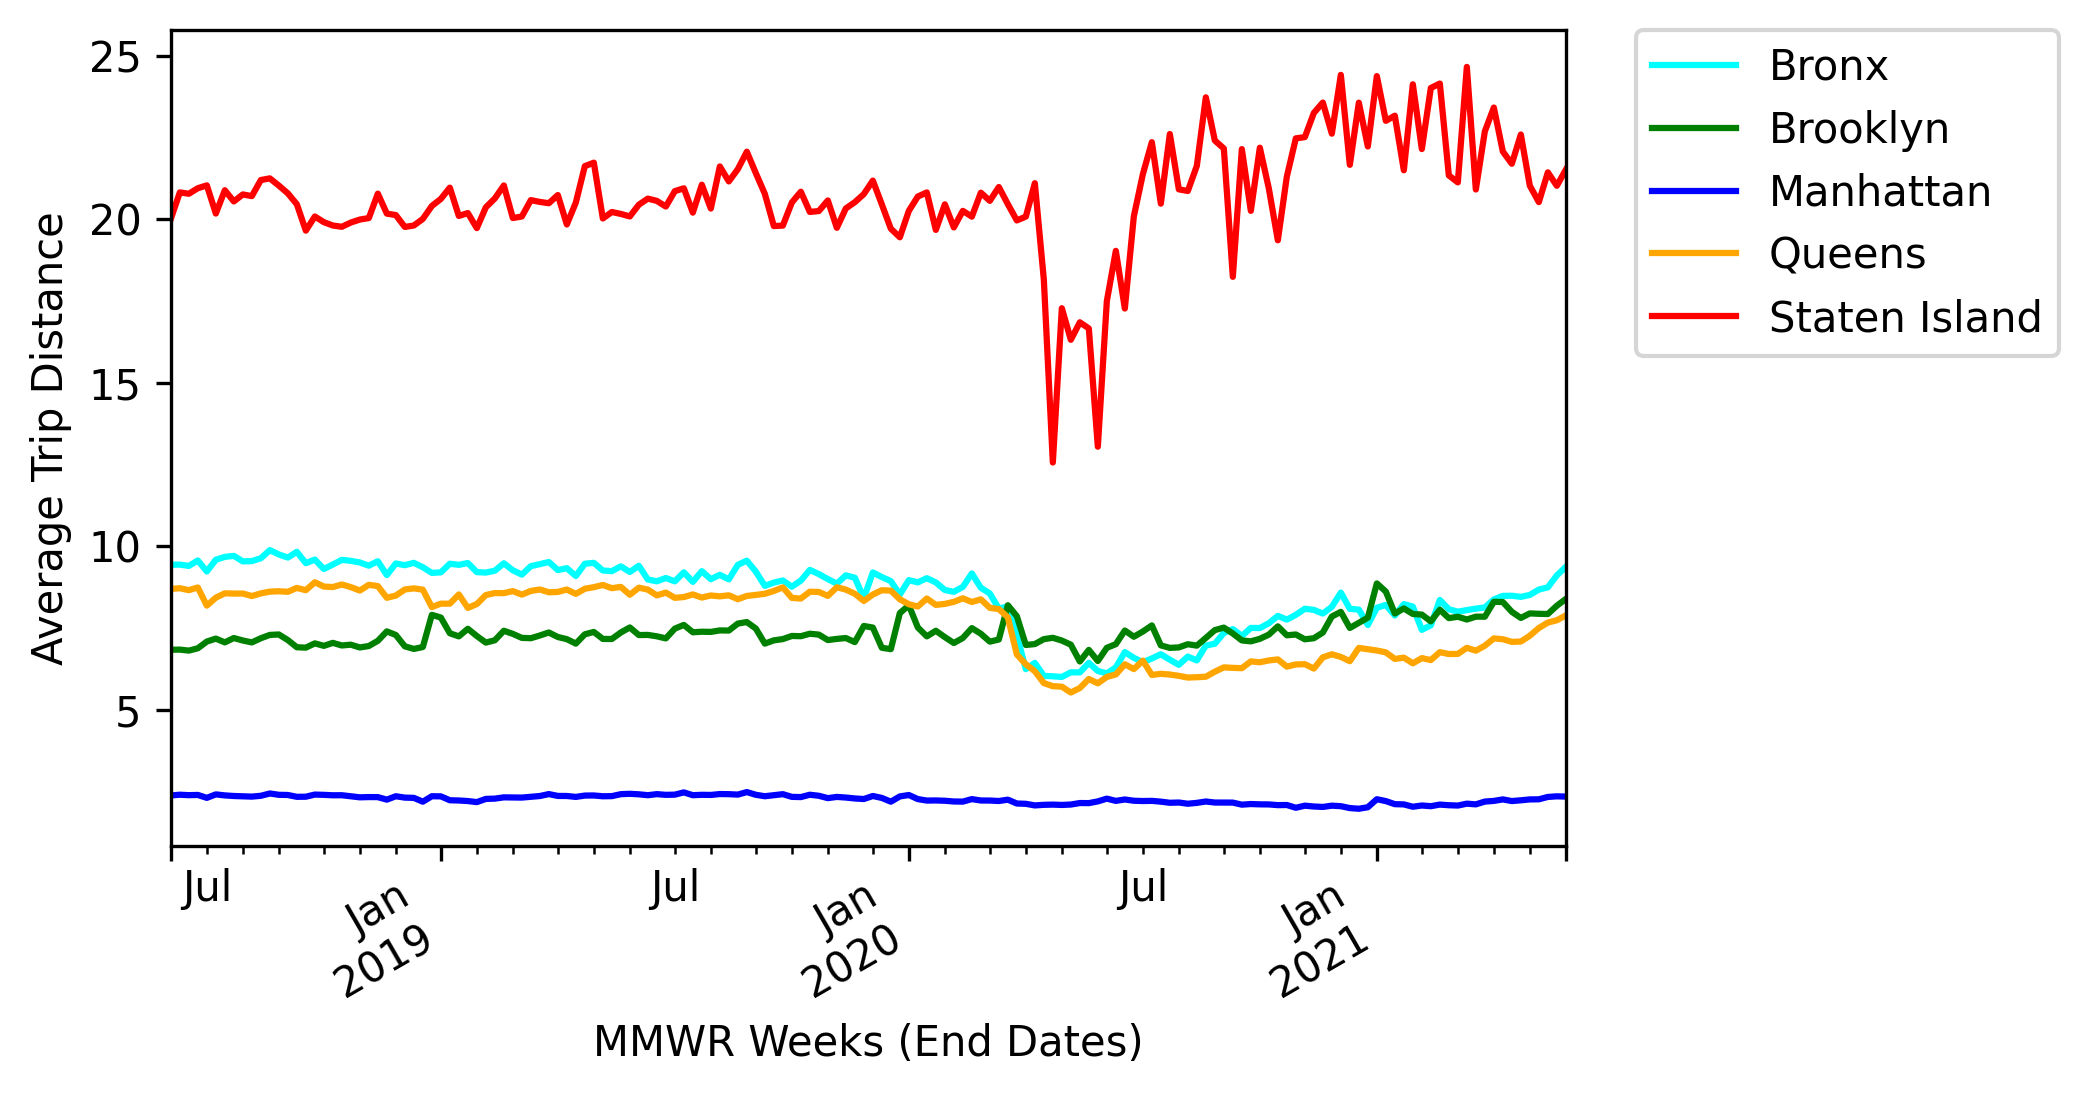
\includegraphics[width=0.45\textwidth]{../plots/time-series-Average Trip Distance-vs-MMWR Weeks (End Dates)-by-do_borough.png}
    %     % this ensures your figures are centered where possible
    %     \label{fig:ts}
    % \end{figure}
% \end{multicols}

% % This uptick in travel distance is likely caused by reduced usage of the Staten Island ferry and the reduced schedule during the pandemic \cite{dot2020}.
% % If this is the case, then Figure~\ref{fig:ts} suggests that people travelling to and from Staten Island rely on taxis to be safer and ontime over the ferry service.
% % The trip distances between boroughs are generally not very homoegeneous. 
% % A likely reason for this heterogeneity is the difference in commutes to work, since
% % many jobs are likely located in Manhattan.

% \begin{multicols}{2}

    This may also come as a result of Staten Island's separation from the other boroughs
    contributing to many possible factors.
    Something as simple as culture could play a roles in differentiating the travel patterns between boroughs.

    Figure~\ref{fig:ts} shows the variation in COVID-19 and Influenza cases per 100'000 people over time.
    One obvious limitation of both datasets is they look very skewed towards the lower values,
    meaning there will be many datapoints with small case rates, and very few points with larger case rates.
    This kind of skew suggests that some points of data will have higher leverage when fitting models than others,
    making the above cleaning and outlier removal processes crucial.
    Both datasets have spikes of case rates, but COVID-19 experiences a significant jump in January 2022.
    
    \begin{figure}[H]

        \centering

        % change the scale multiplier to make the figures smaller or larger
        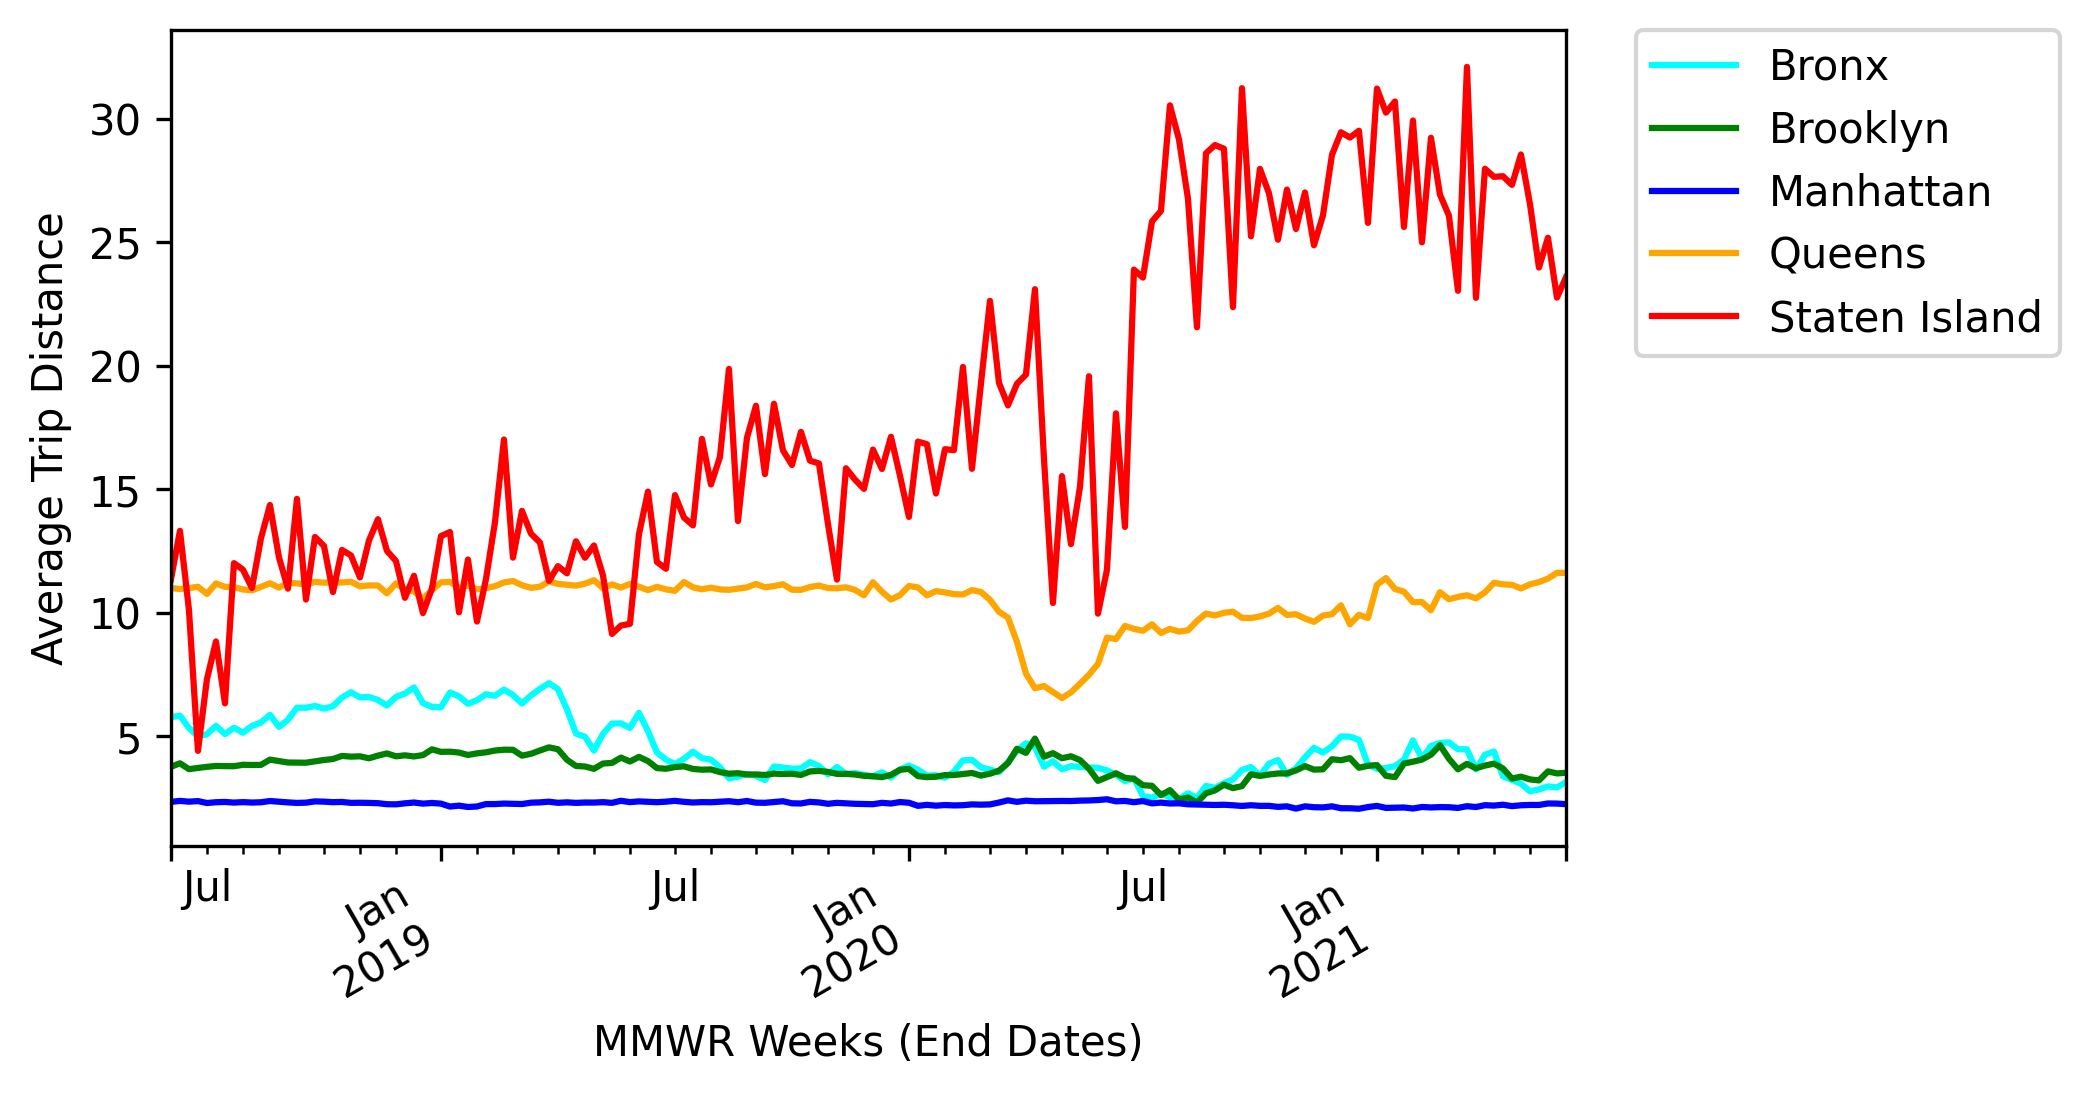
\includegraphics[width=0.58\textwidth]{../plots/time-series-Average Trip Distance-vs-MMWR Weeks (End Dates)-by-pu_borough.png}
        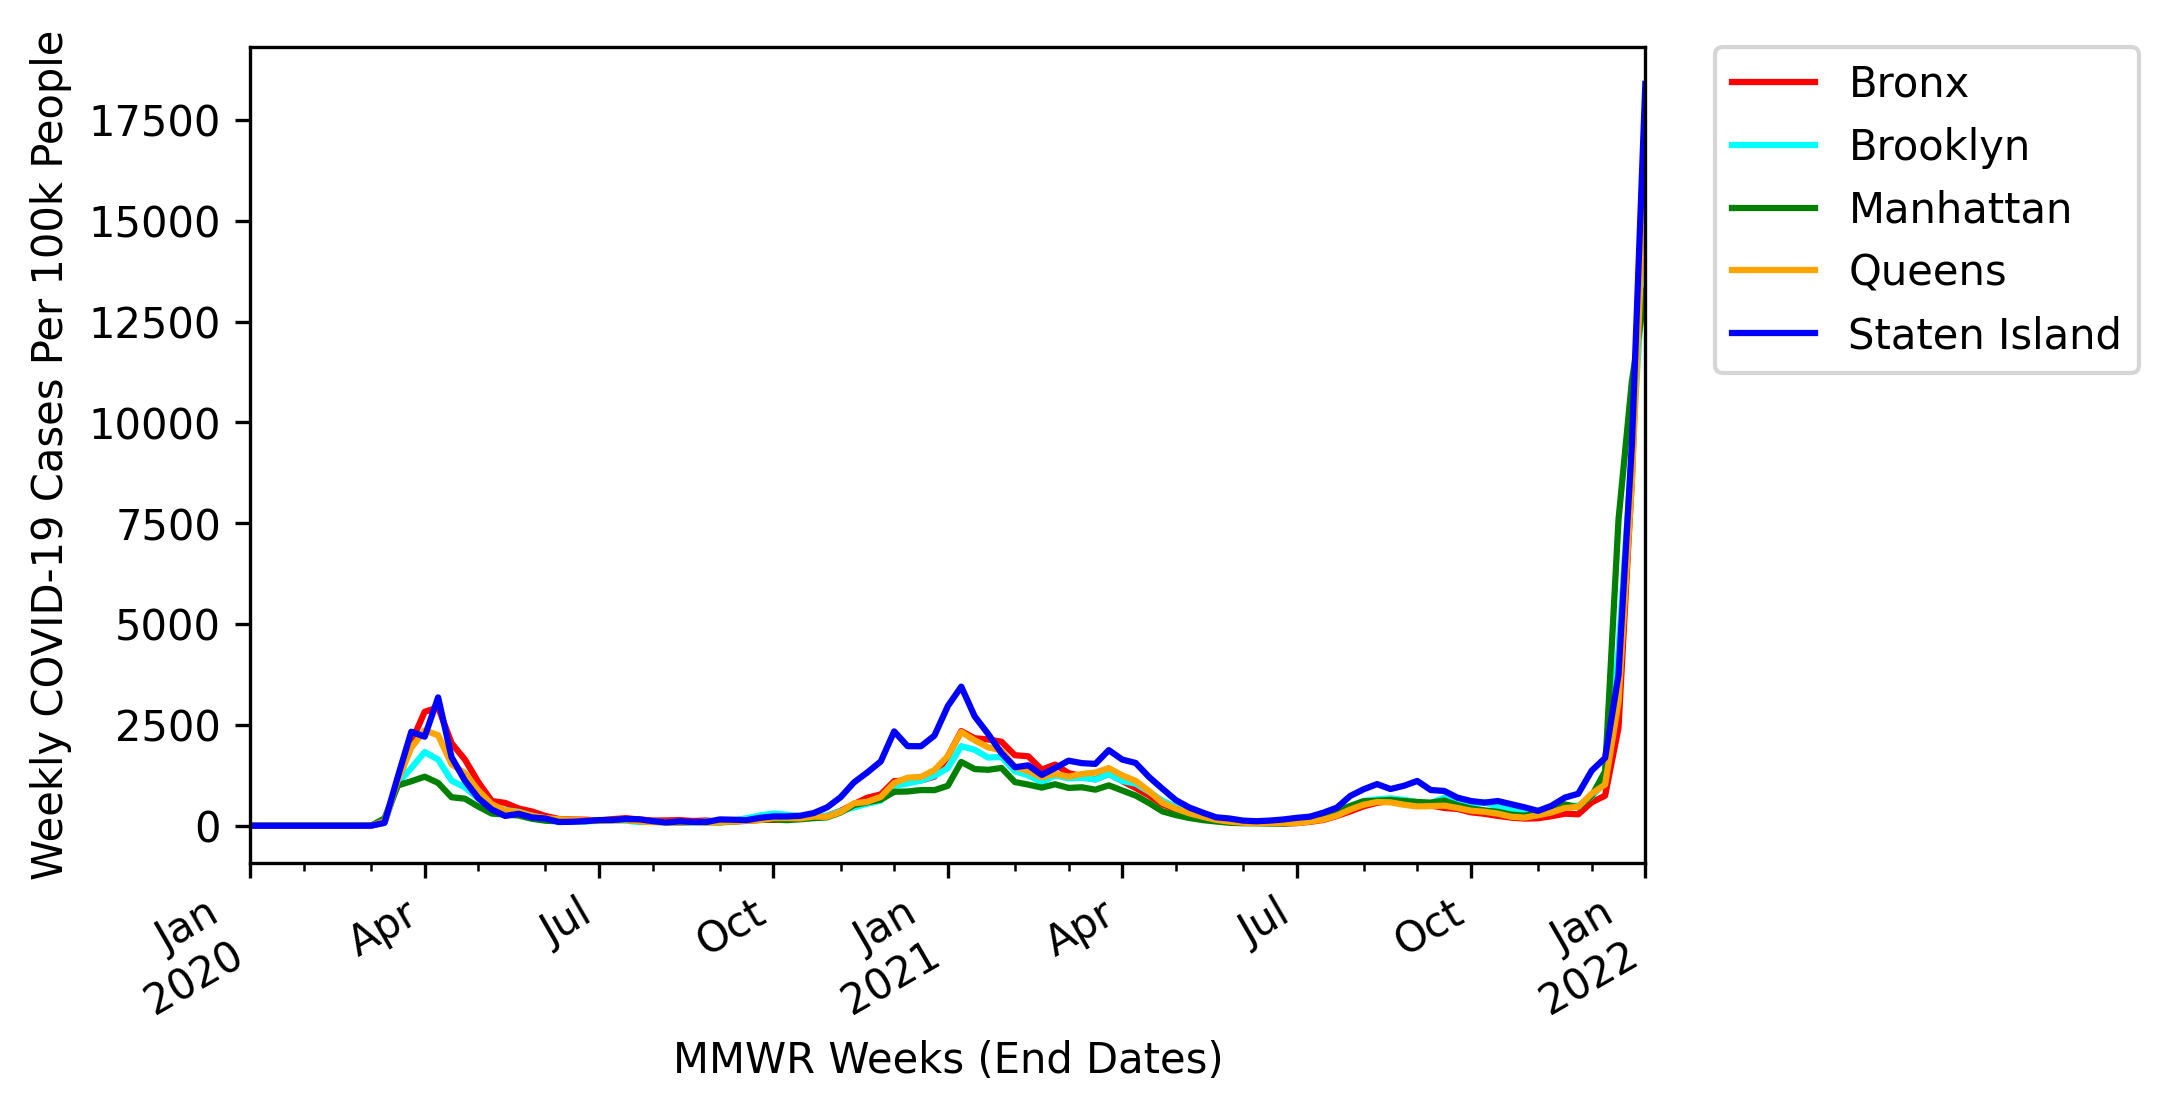
\includegraphics[width=0.58\textwidth]{../plots/time-series-Weekly COVID-19 Cases Per 100k People-vs-MMWR Weeks (End Dates)-by-borough.png}
        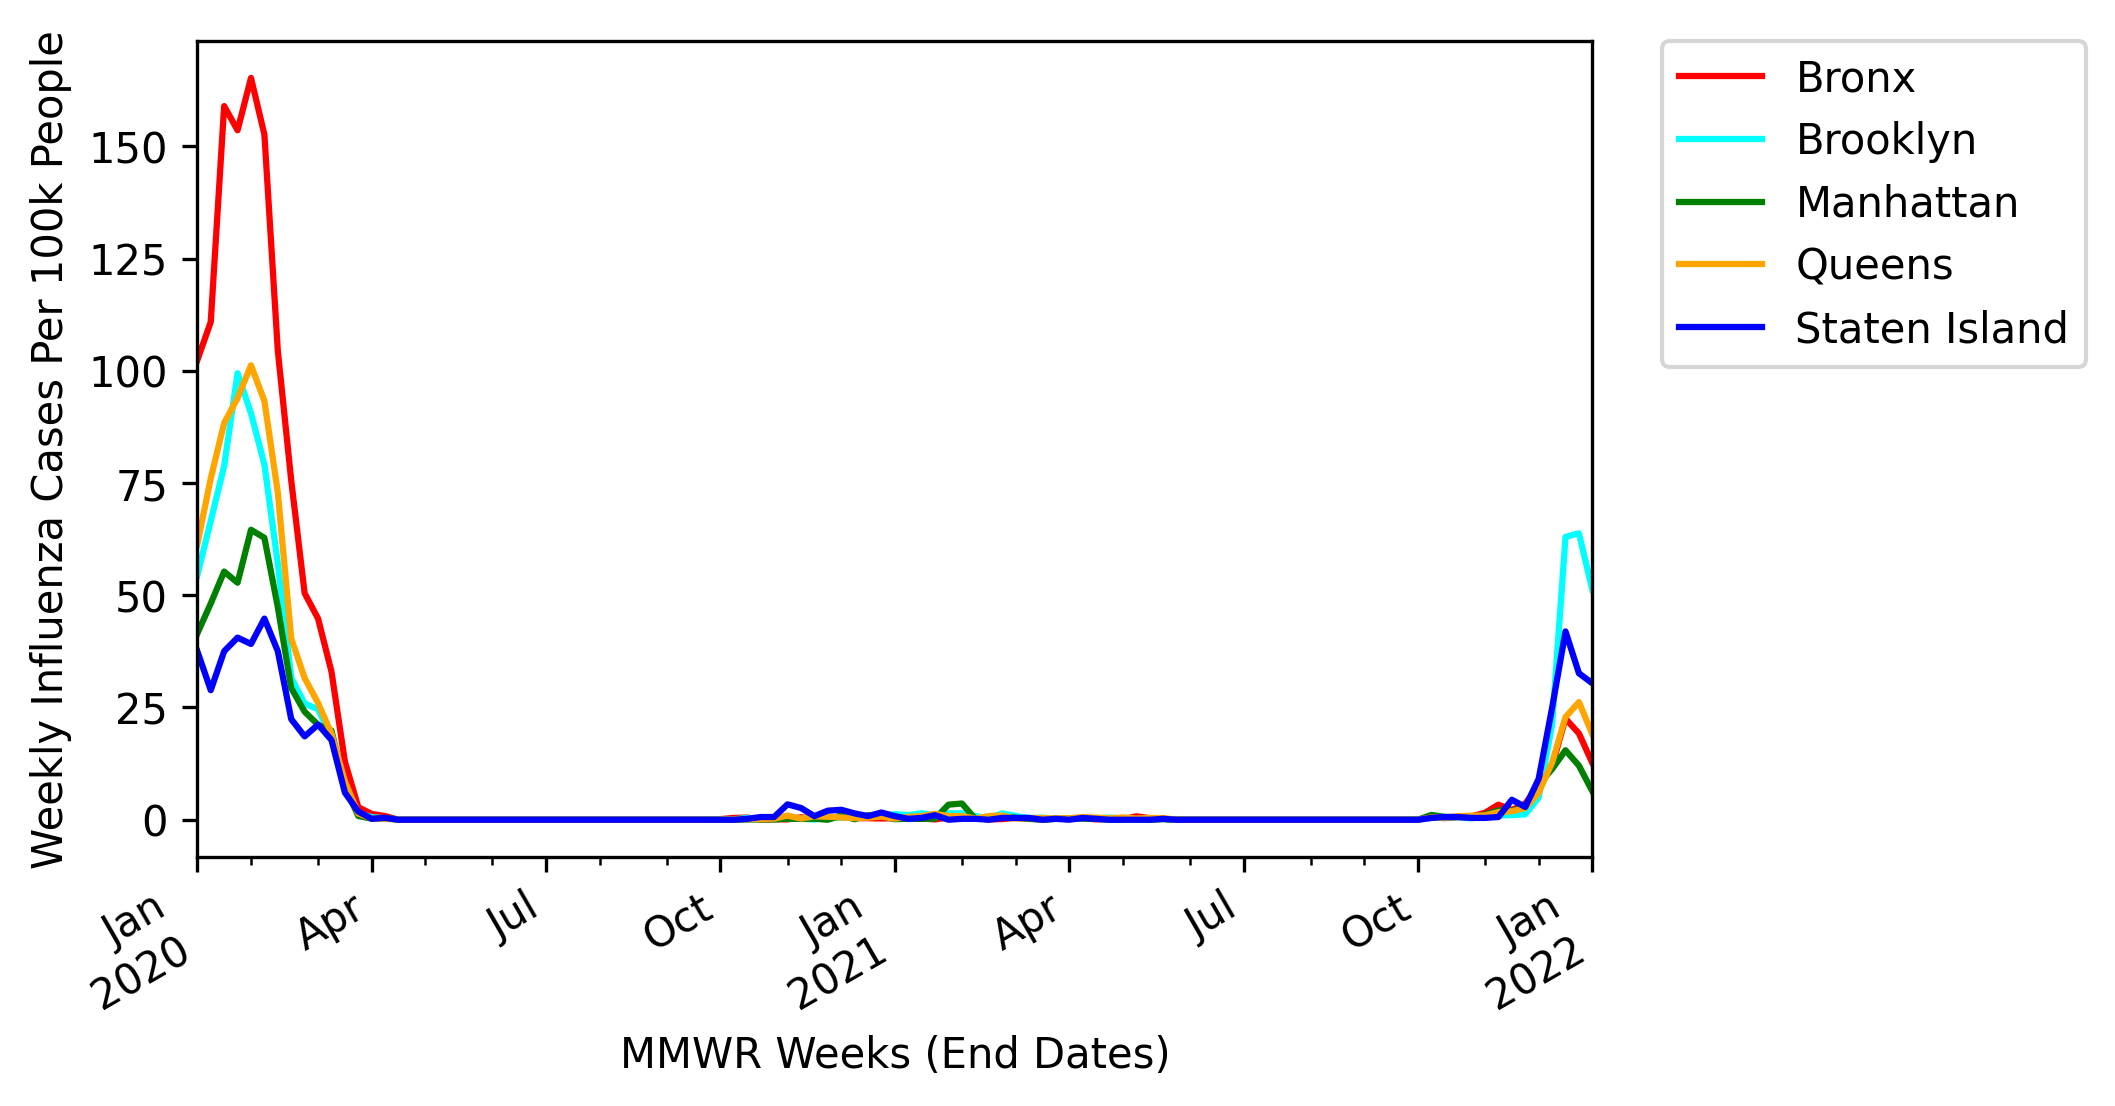
\includegraphics[width=0.58\textwidth]{../plots/time-series-Weekly Influenza Cases Per 100k People-vs-MMWR Weeks (End Dates)-by-borough.png}
        \caption{How Average Trip Distances (top), COVID-19 (middle) and Influenza (bottom) case counts per 100k people vary over time.} % refer to this image as (Figure 1)

        % 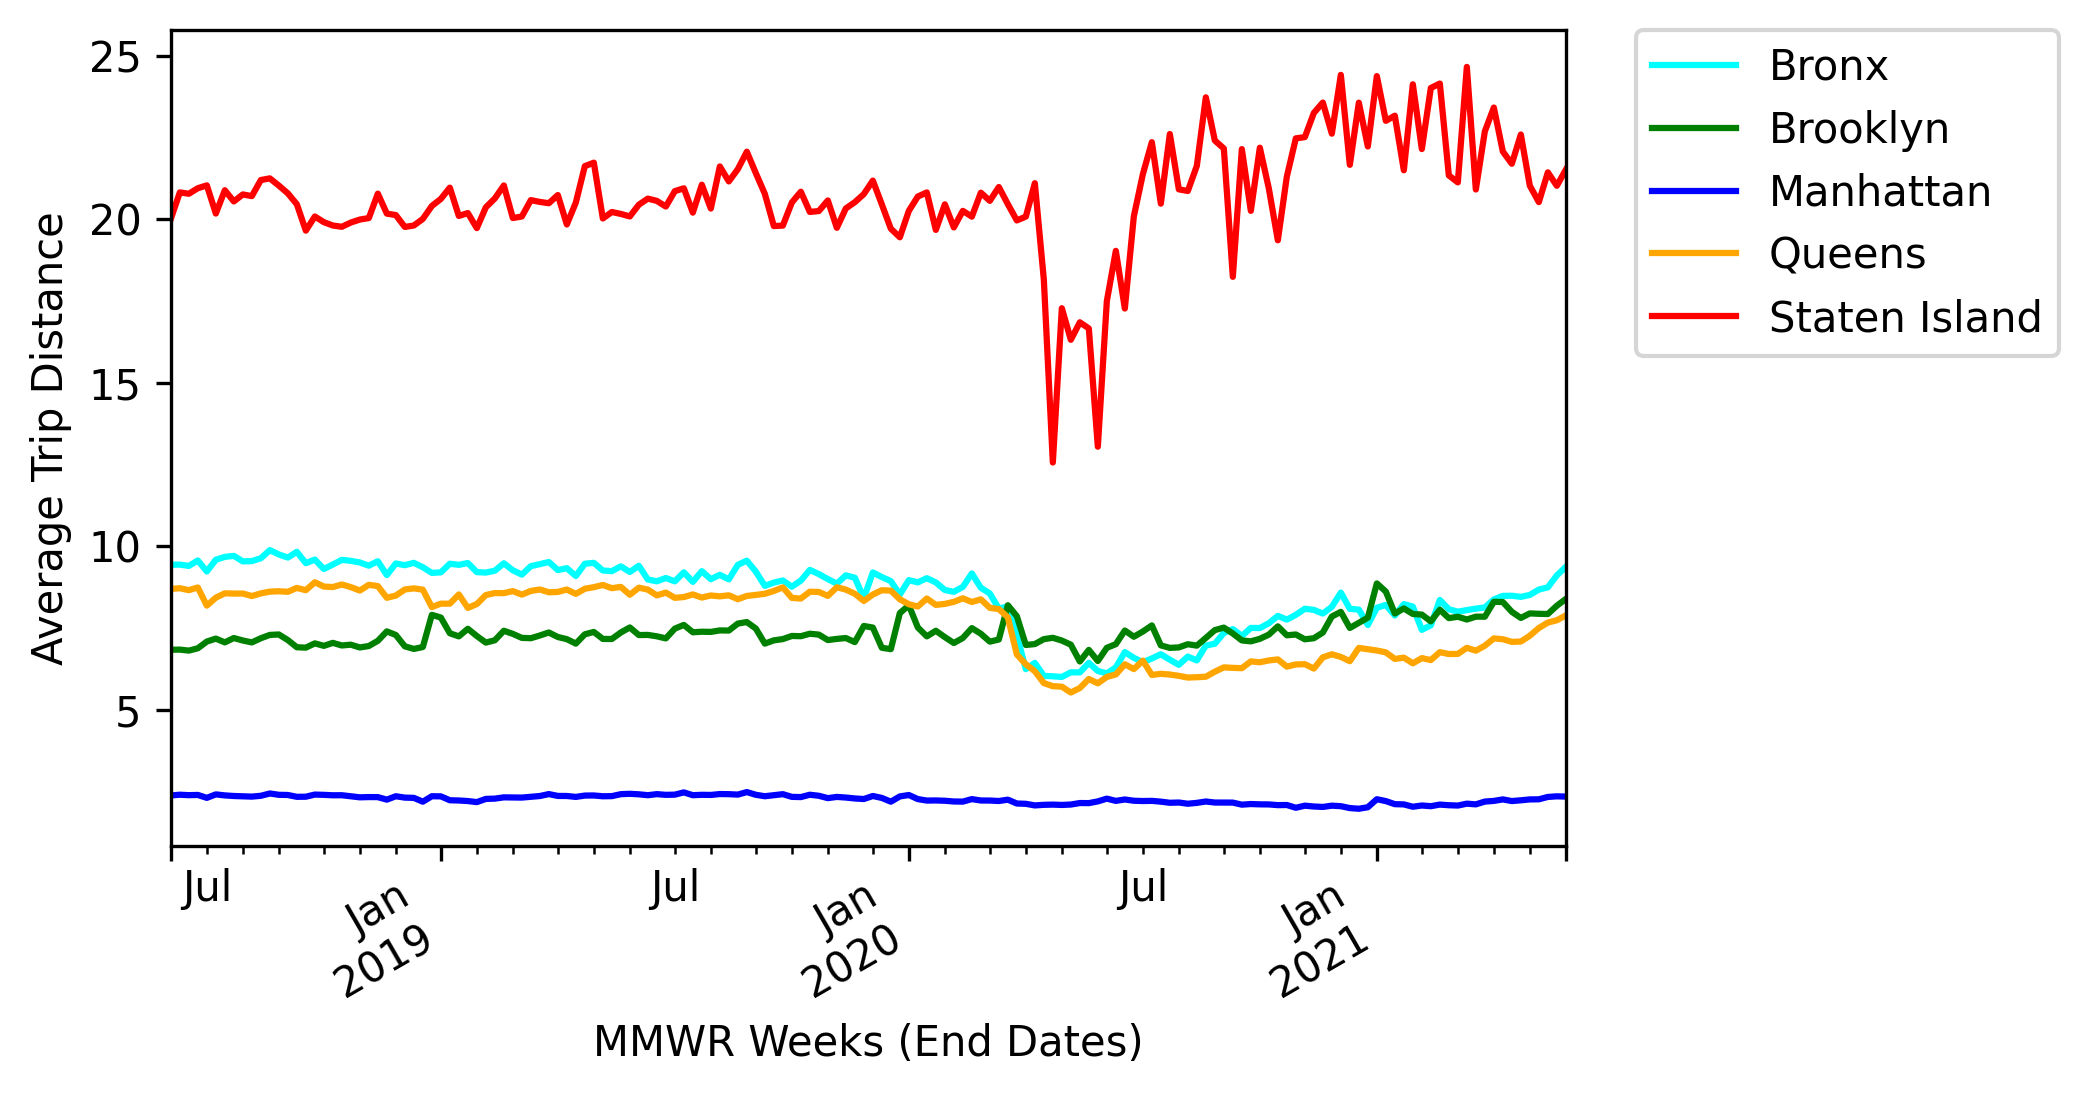
\includegraphics[width=0.45\textwidth]{../plots/time-series-Average Trip Distance-vs-MMWR Weeks (End Dates)-by-do_borough.png}
        % this ensures your figures are centered where possible
        \label{fig:ts}
    \end{figure}

\end{multicols}
    

% \end{multicols}

% \begin{wrapfigure}{r}{8cm}
%     % change the scale multiplier to make the figures smaller or larger
%     \caption{How average trip distances per week per pick-up borough vary over time.} % refer to this image as (Figure 1)
%     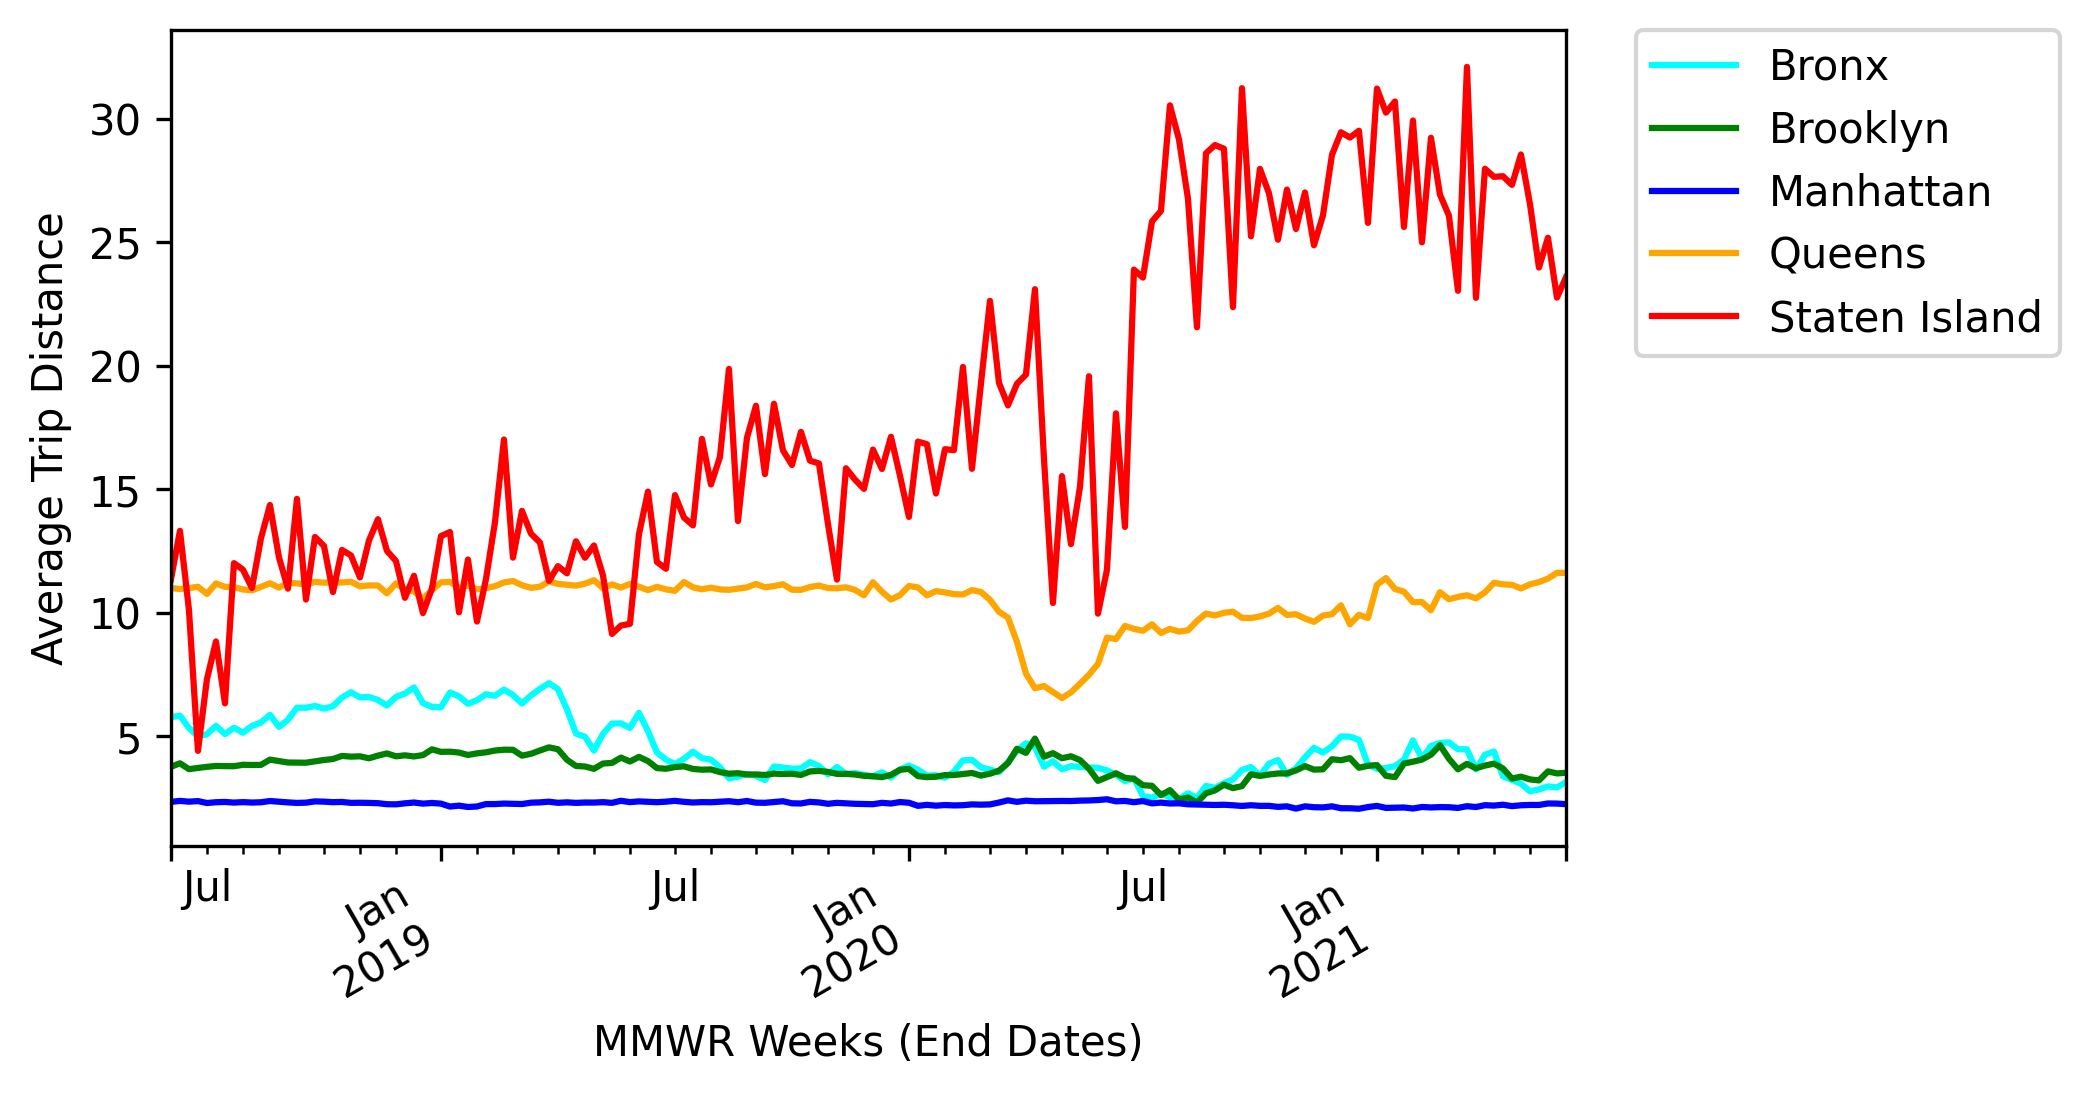
\includegraphics[width=0.55\textwidth]{../plots/time-series-Average Trip Distance-vs-MMWR Weeks (End Dates)-by-pu_borough.png}

%     % 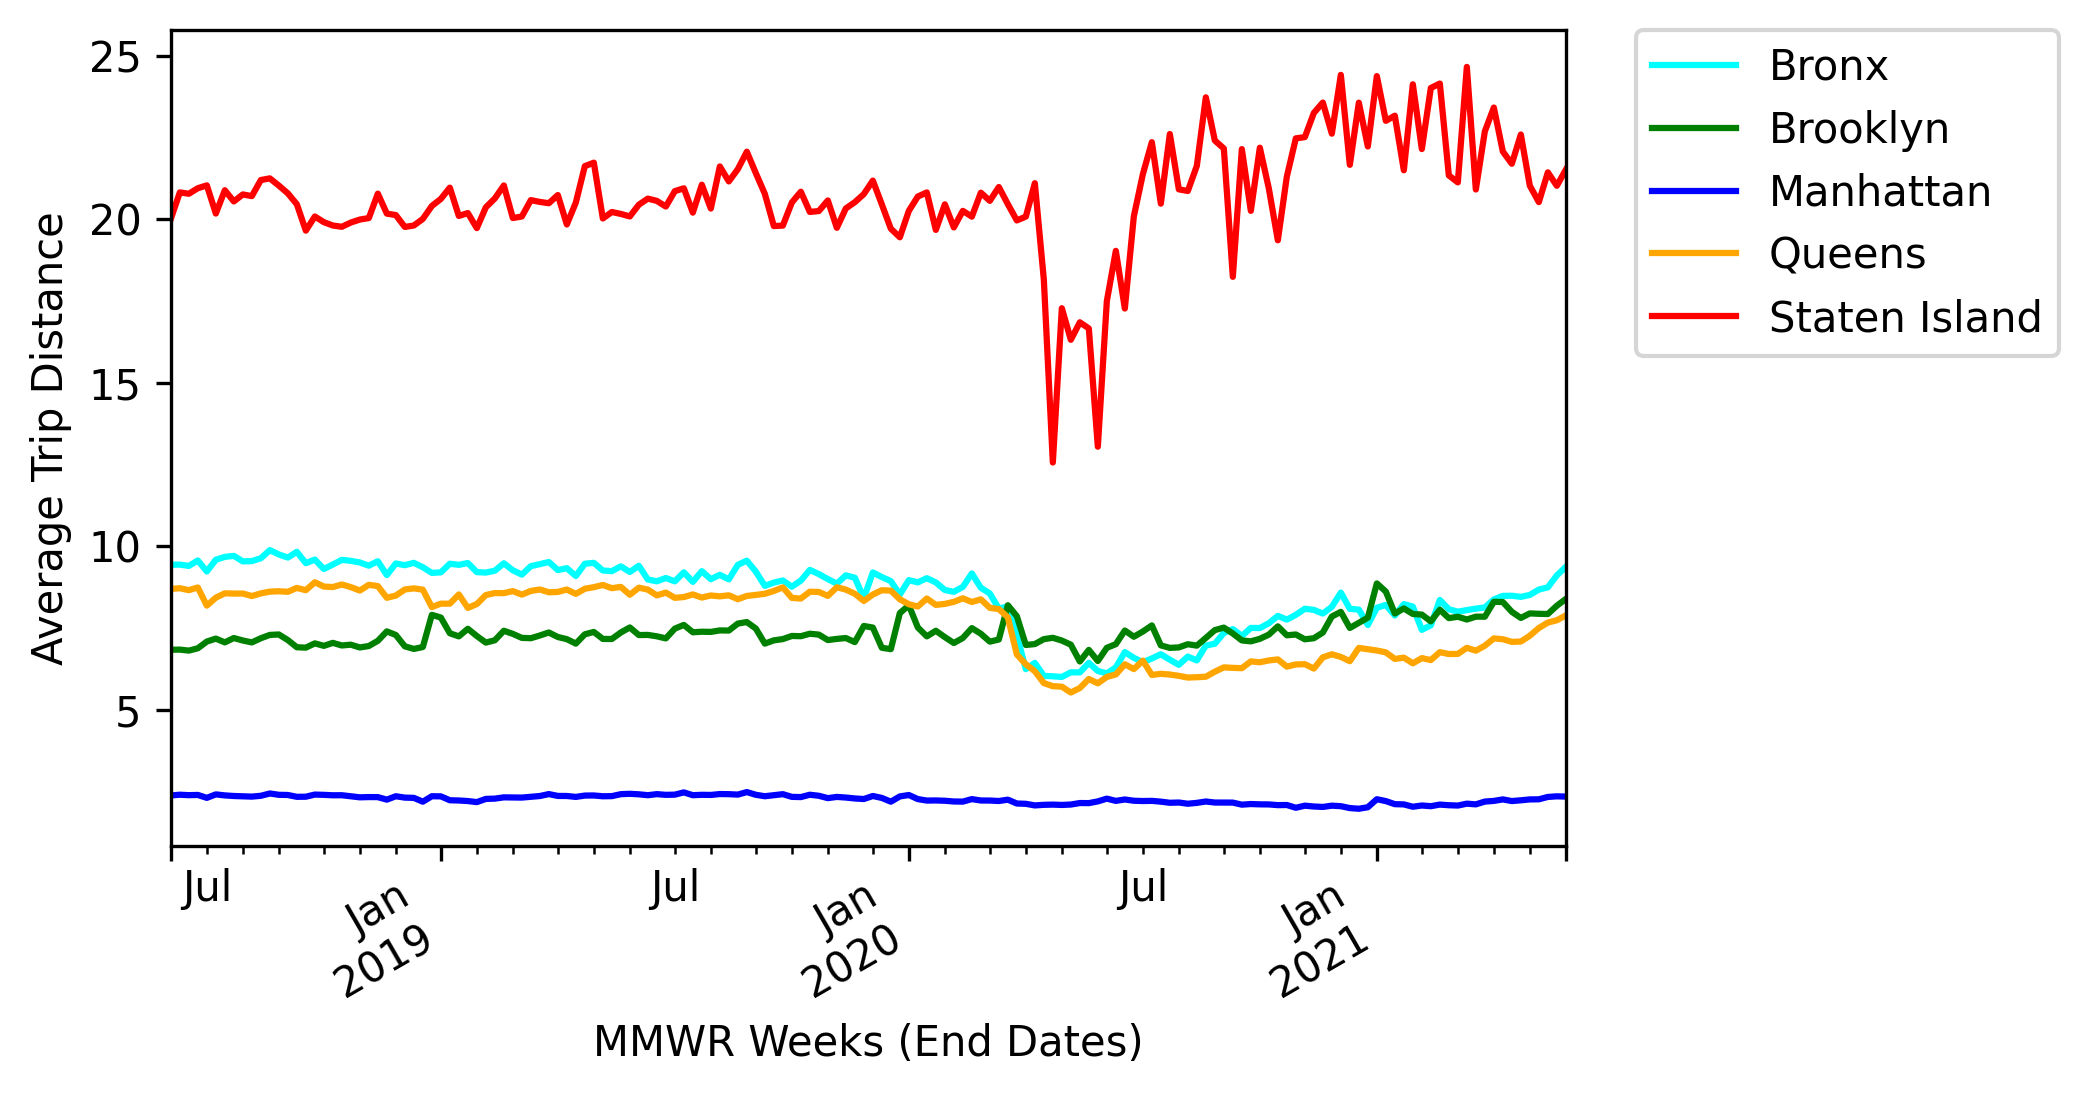
\includegraphics[width=0.45\textwidth]{../plots/time-series-Average Trip Distance-vs-MMWR Weeks (End Dates)-by-do_borough.png}
%     % this ensures your figures are centered where possible
%     % \centering
%     \label{fig:ts}
% \end{wrapfigure}


% \begin{wrapfigure}{r}{5.5cm}
%     % change the scale multiplier to make the figures smaller or larger
%     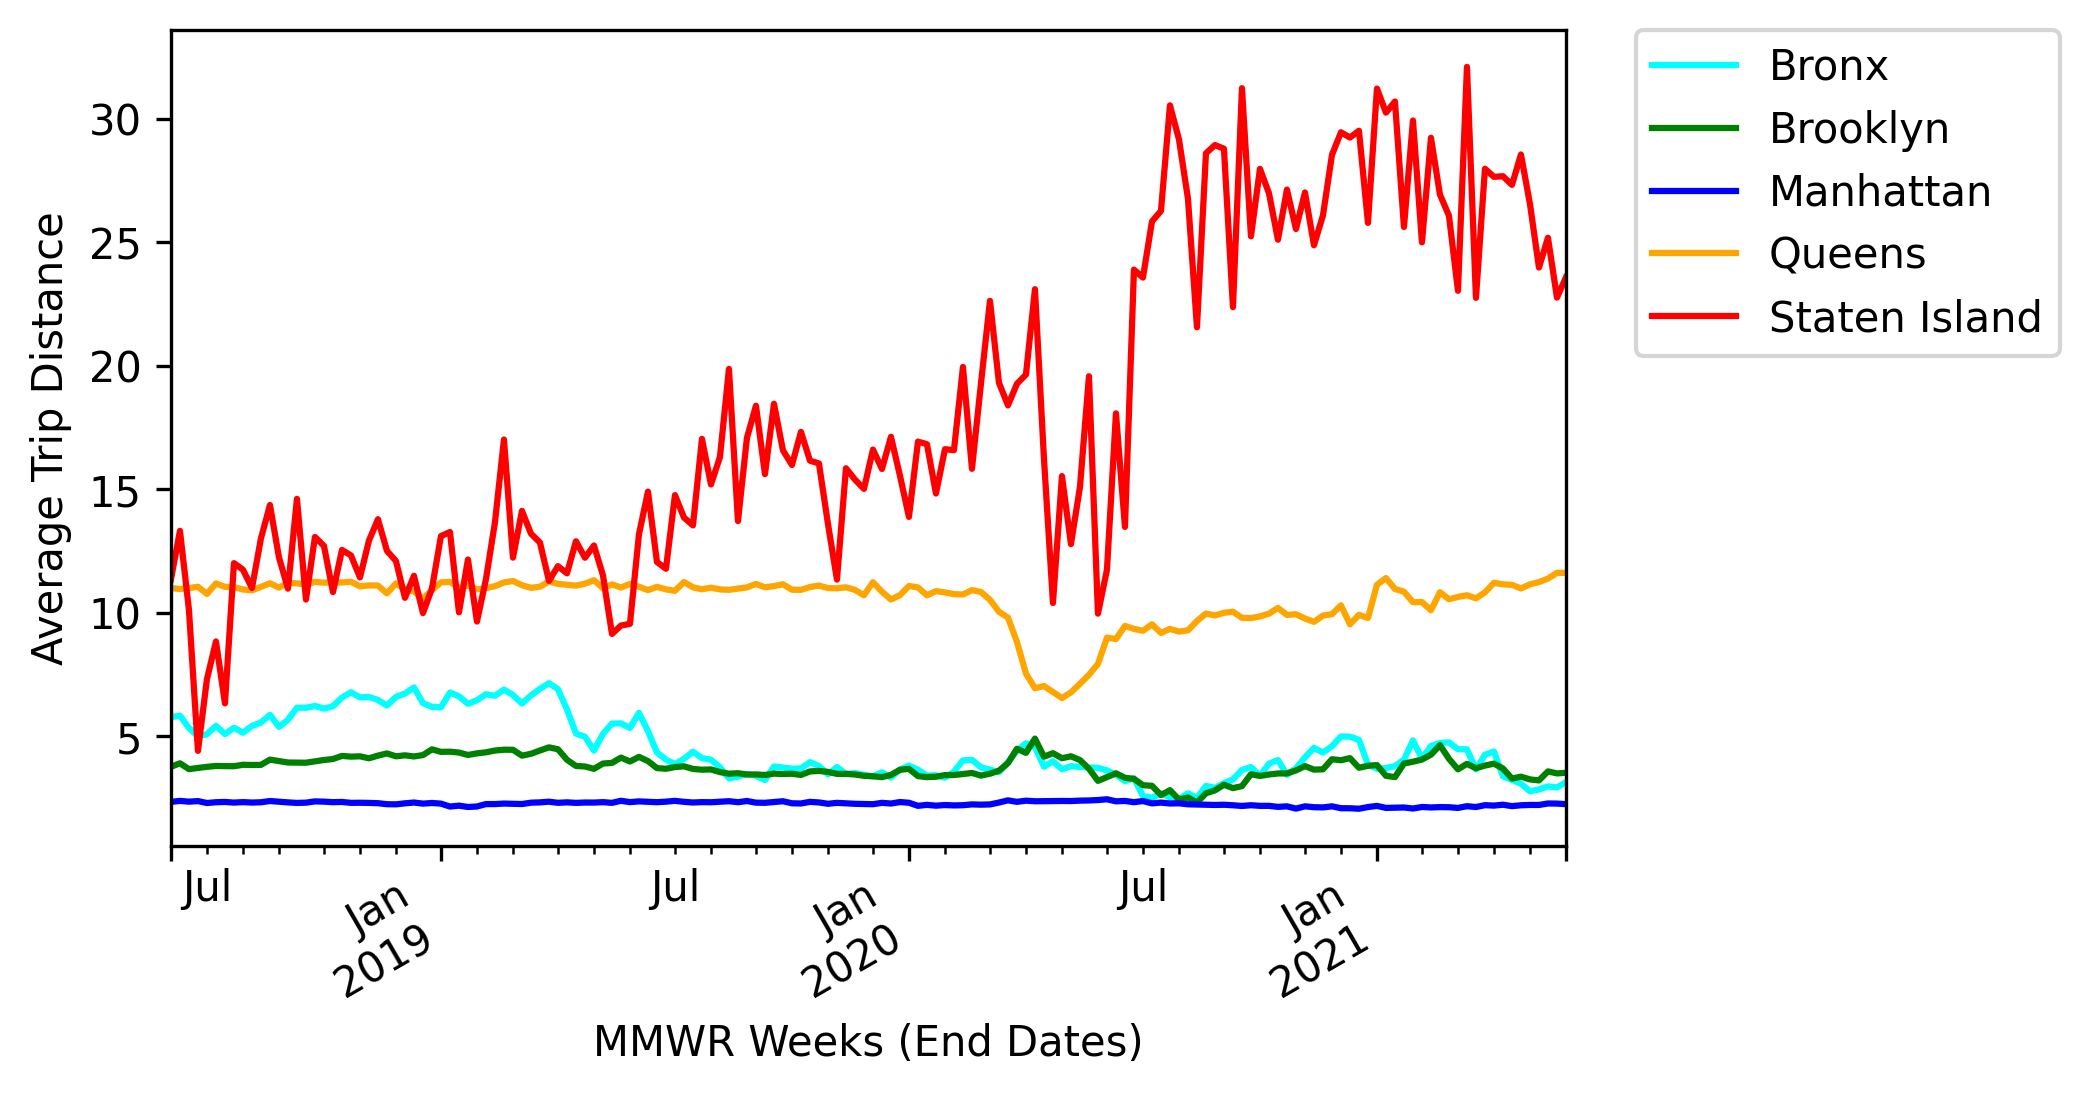
\includegraphics[width=0.55\textwidth]{../plots/time-series-Average Trip Distance-vs-MMWR Weeks (End Dates)-by-pu_borough.png}

%     % 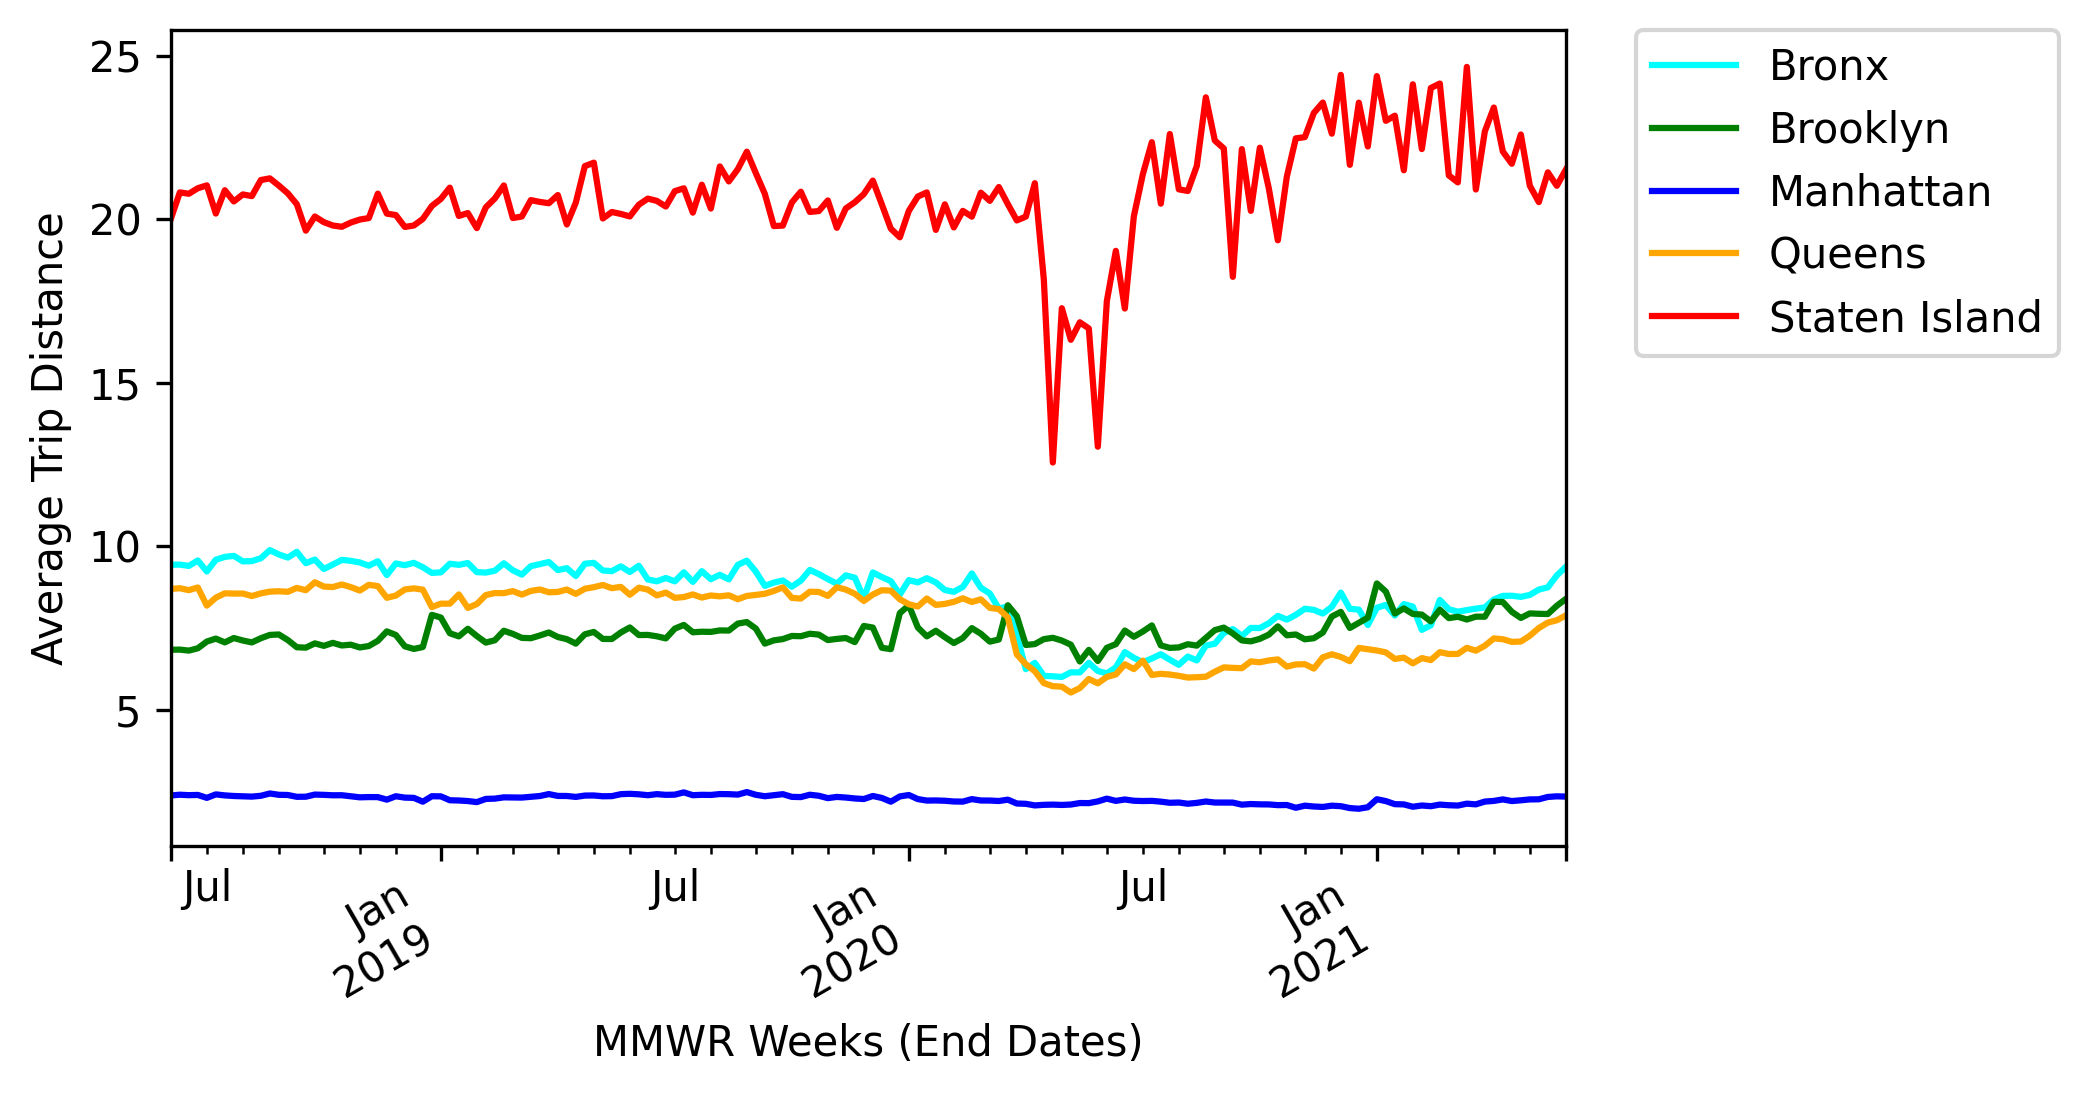
\includegraphics[width=0.45\textwidth]{../plots/time-series-Average Trip Distance-vs-MMWR Weeks (End Dates)-by-do_borough.png}
%     % this ensures your figures are centered where possible
%     \centering
%     \caption{How average trip distances per week per pick-up borough vary over time.} % refer to this image as (Figure 1)
%     \label{fig:ts}
% \end{wrapfigure}

% \end{multicols}

% \begin{wrapfigure}{r}{8cm}

%     % this ensures your figures are centered where possible
%     \centering

%     % change the scale multiplier to make the figures smaller or larger
%     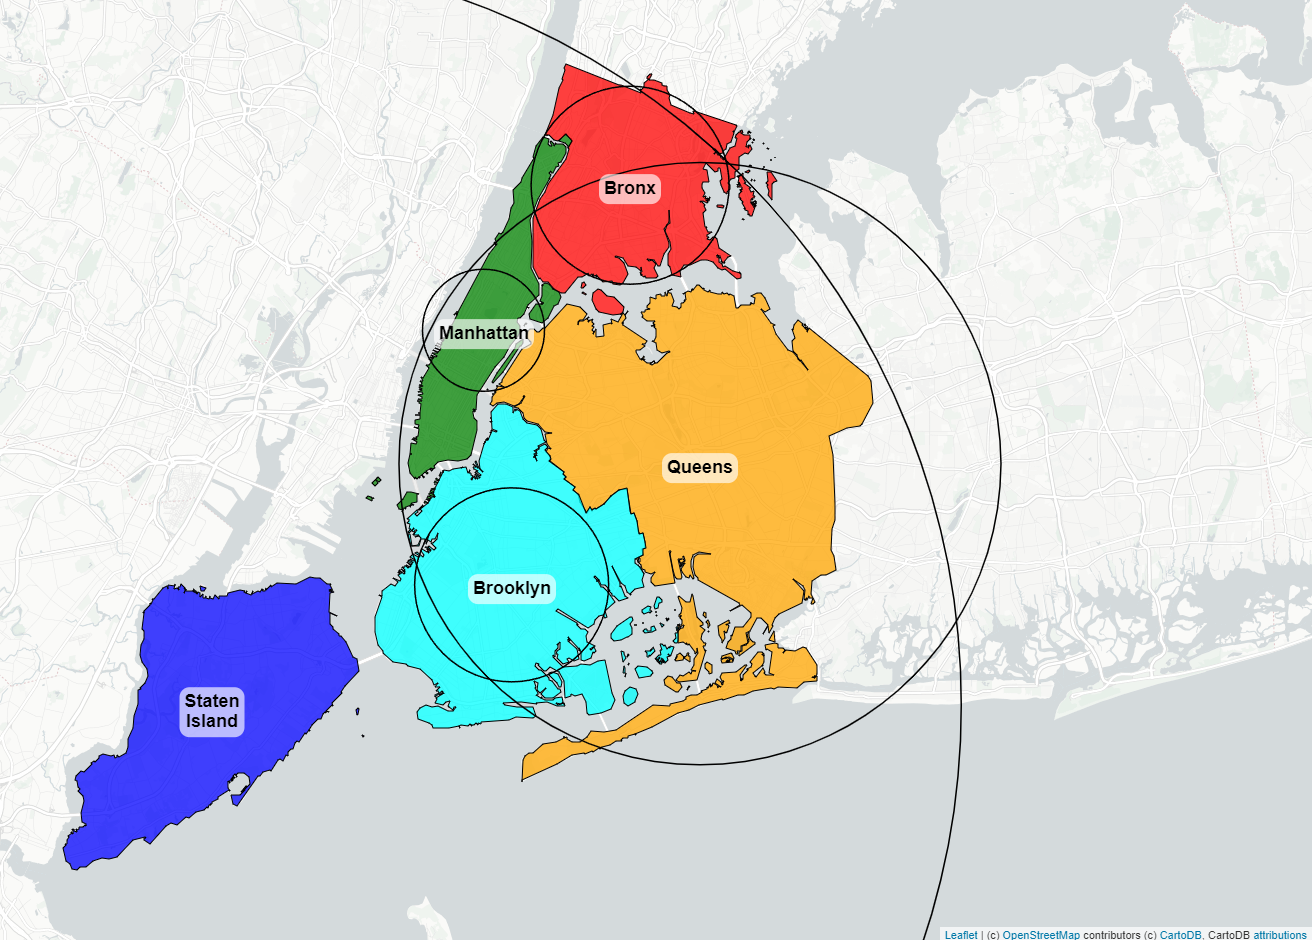
\includegraphics[width=0.5\textwidth]{../plots/map-avg-trip-distance-overall-pu_borough-MODIFIED.png}

%     \caption{Map of average trip distance overall.} 
%     % refer to this image as (Figure 1)
%     \label{map:overall}
% \end{wrapfigure}


% \begin{figure}[h]
%     % change the scale multiplier to make the figures smaller or larger
%     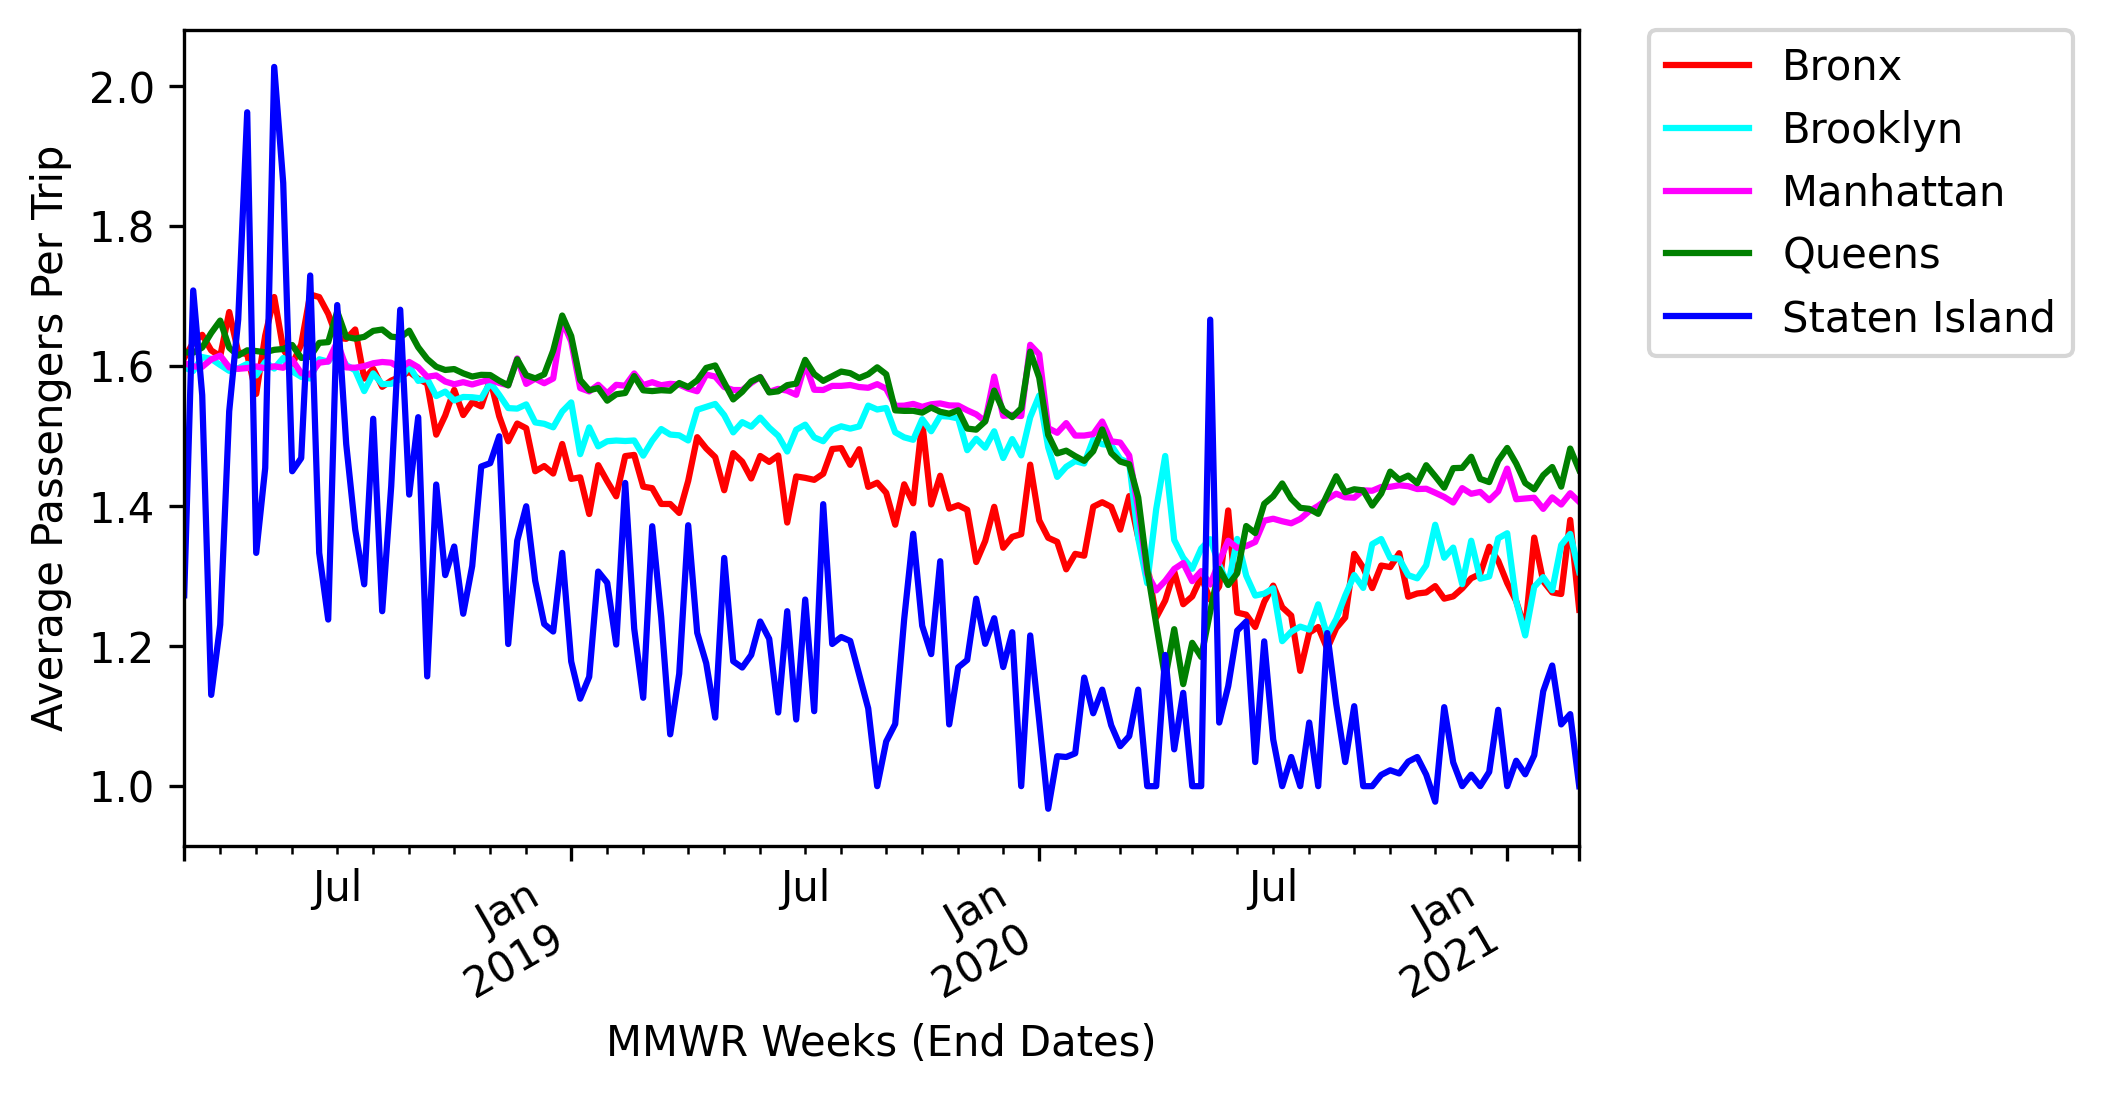
\includegraphics[width=0.45\textwidth]{../plots/time-series-Average Passengers Per Trip-vs-MMWR Weeks (End Dates)-by-pu_borough.png}
%     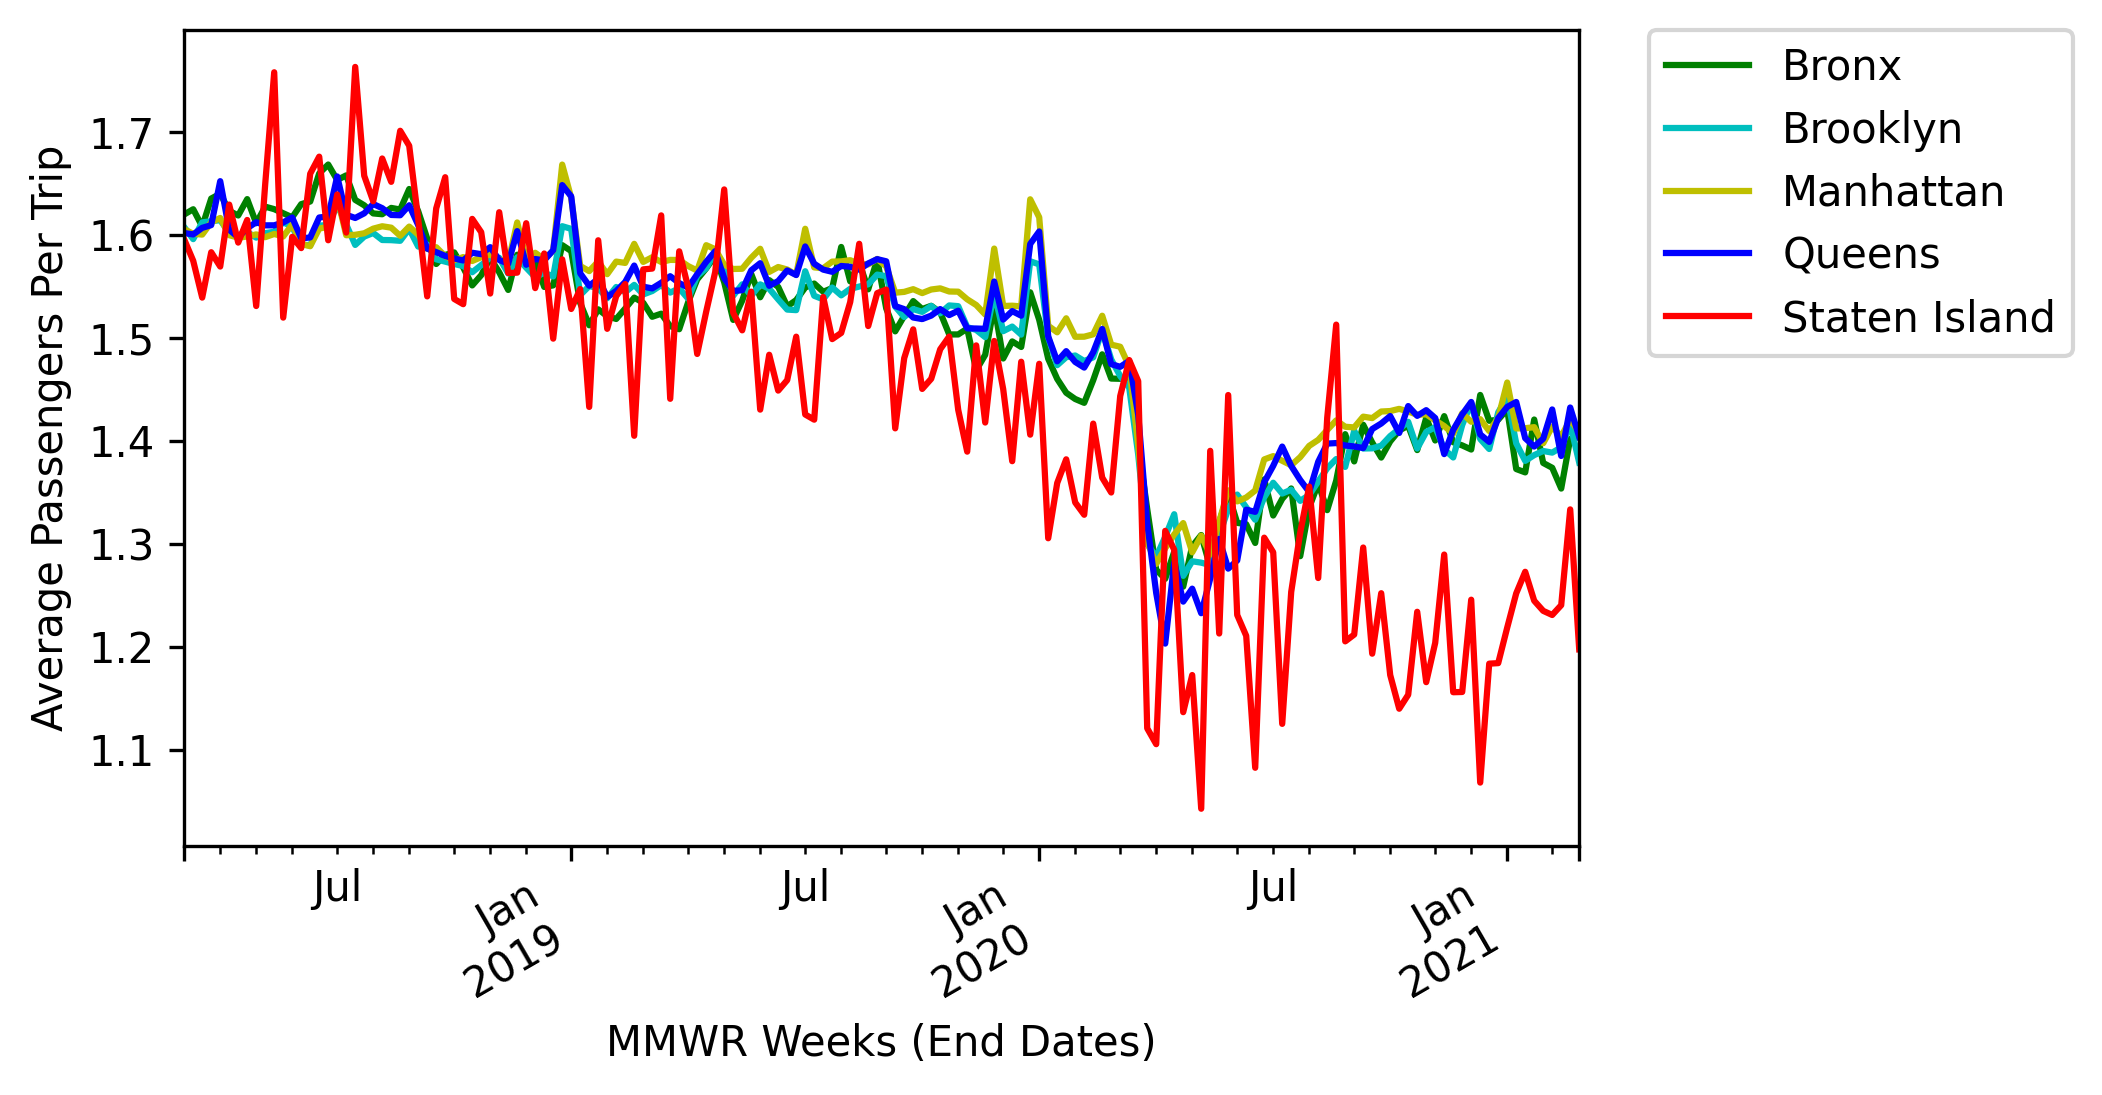
\includegraphics[width=0.45\textwidth]{../plots/time-series-Average Passengers Per Trip-vs-MMWR Weeks (End Dates)-by-do_borough.png}
%     % this ensures your figures are centered where possible
%     \centering
%     \caption{How average passenger count per week per pick-up (left) and drop-off (right) borough vary over time.} % refer to this image as (Figure 1)
%     \label{fig:ts-pass-count-weeks}
% \end{figure}


% \begin{figure}[H]
%     % change the scale multiplier to make the figures smaller or larger
%     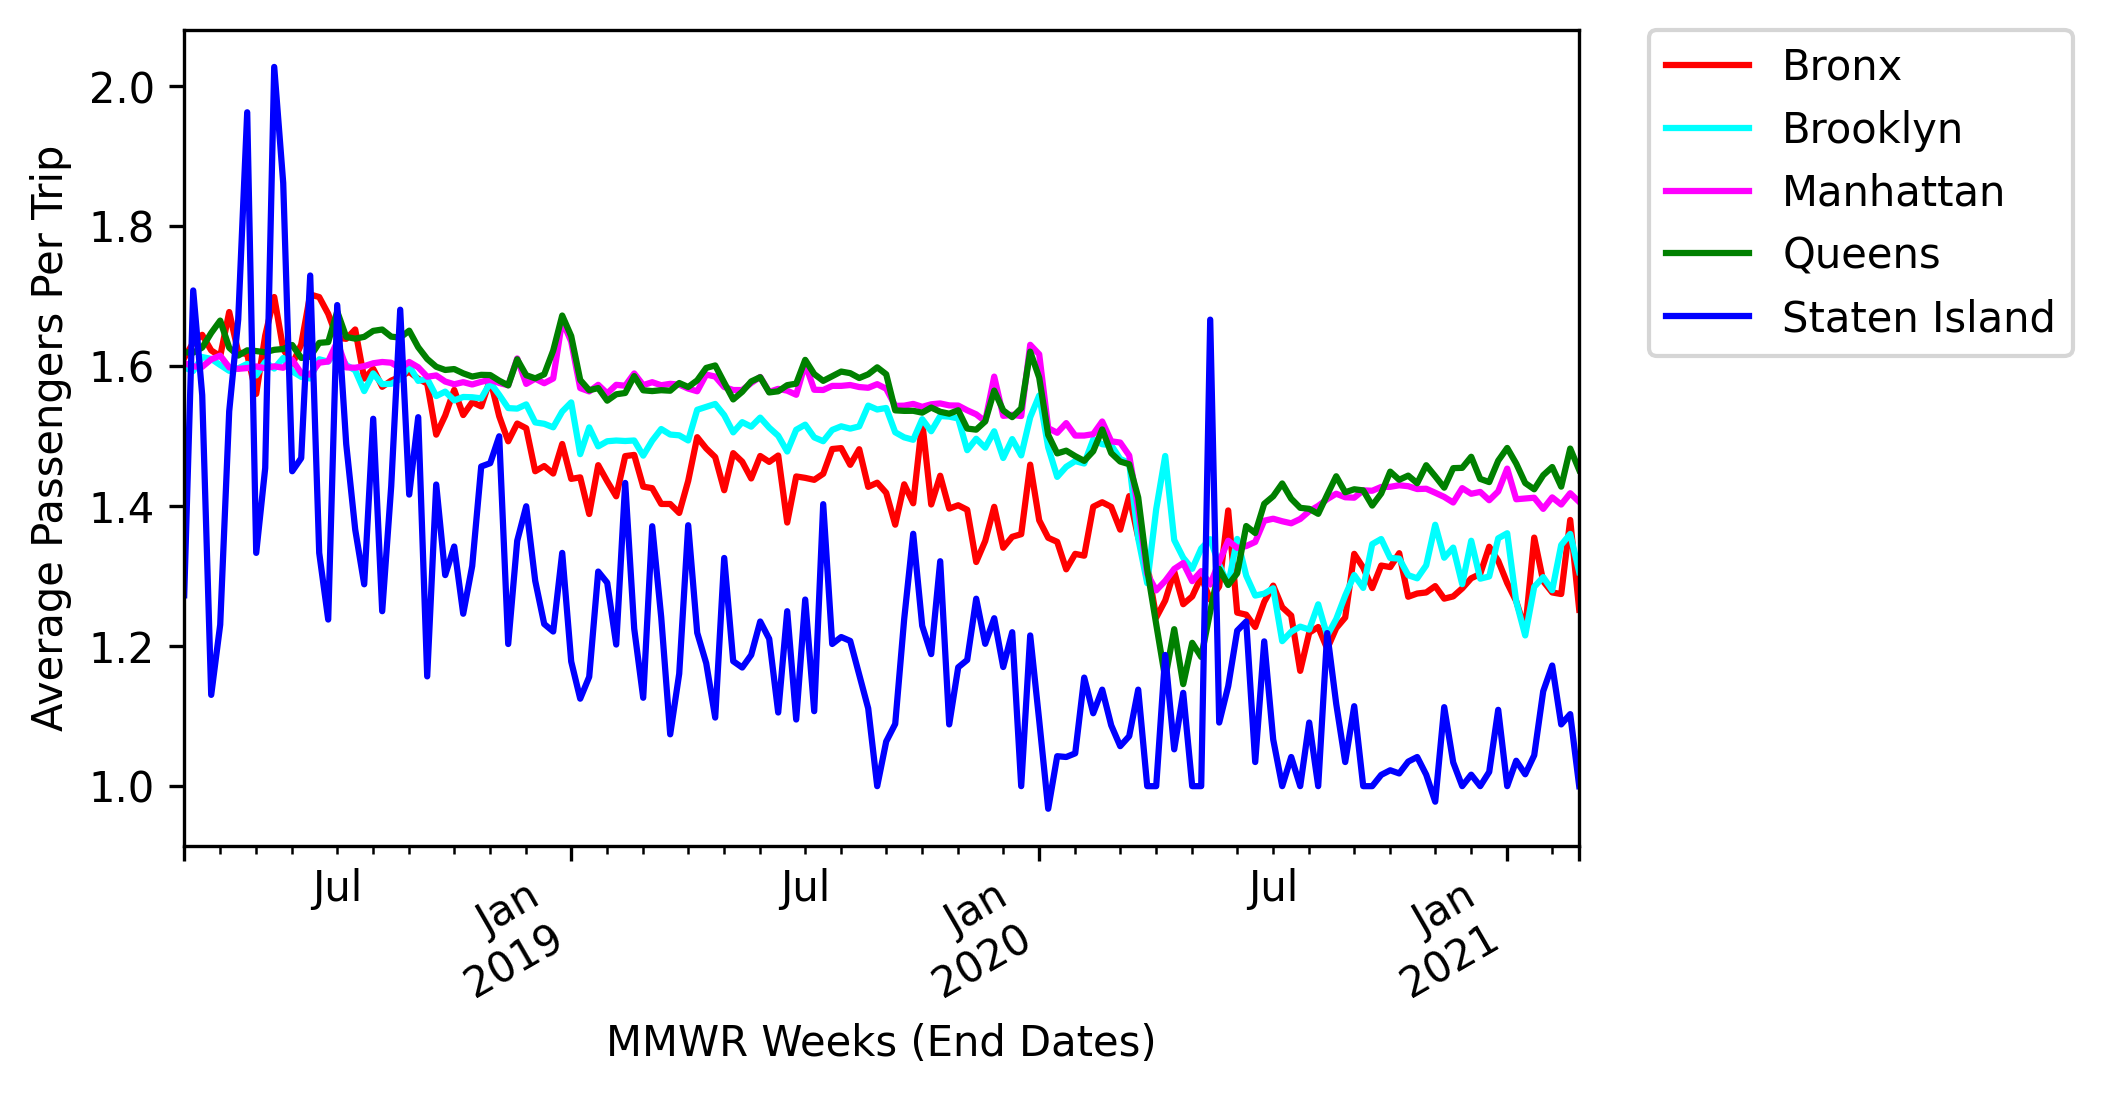
\includegraphics[width=0.5\textwidth]{../plots/time-series-Average Passengers Per Trip-vs-MMWR Weeks (End Dates)-by-pu_borough.png}
%     % 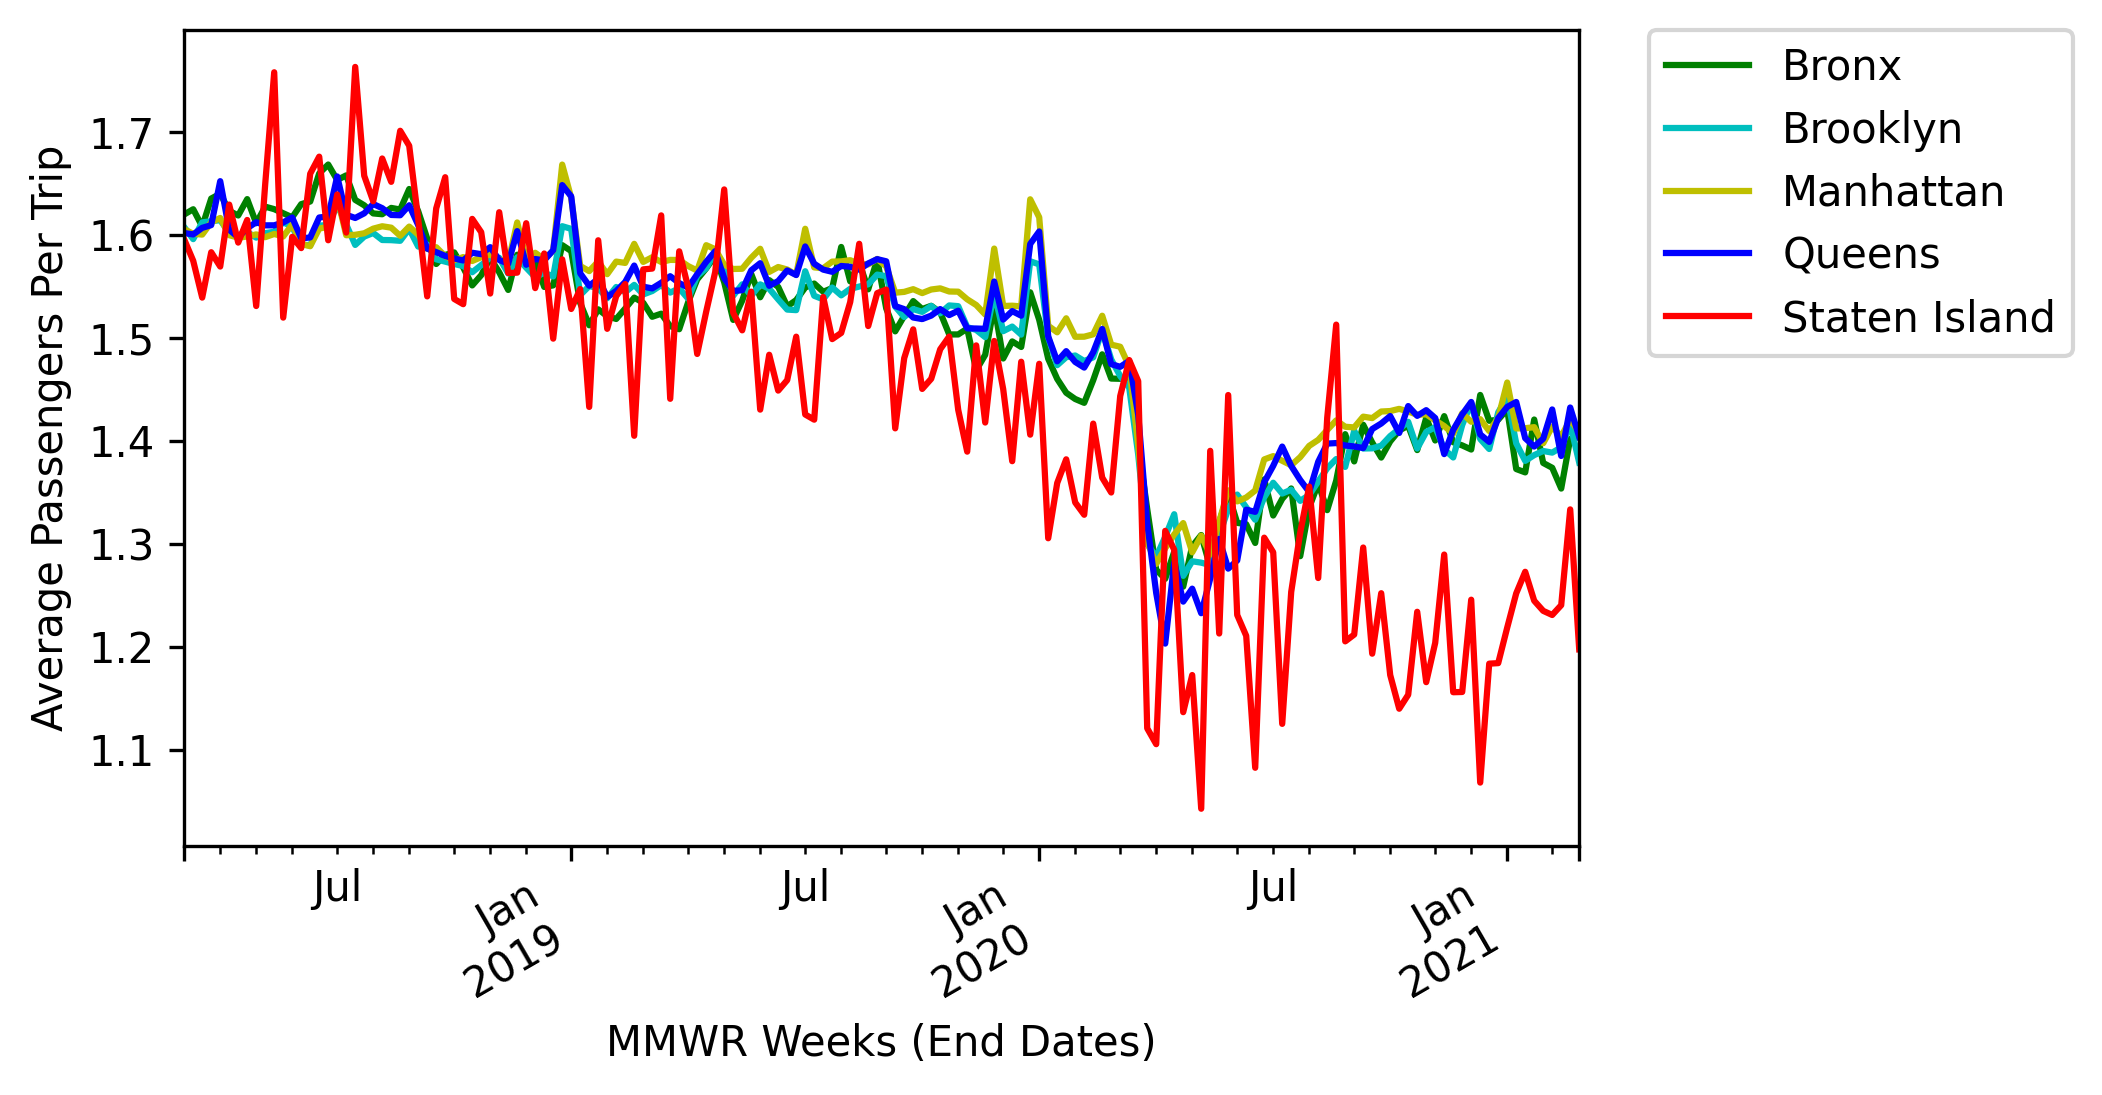
\includegraphics[width=0.45\textwidth]{../plots/time-series-Average Passengers Per Trip-vs-MMWR Weeks (End Dates)-by-do_borough.png}
%     % this ensures your figures are centered where possible
%     \centering
%     \caption{How average passenger counts per week per pick-up borough vary over time.} % refer to this image as (Figure 1)
%     \label{fig:ts-pass-count-weeks}
% \end{figure}

% \begin{multicols}{2}



\textbf{Geospatial Visualisation:}    

While time series plots display variation in average trip distance over time, 
they do not clearly convey the meaning of these differences.
Figures~\ref{map:overall} and \ref{maps} compares the average trip radius overall, 
the average trip radius for the week with maximum COVID-19 cases per capita, 
and the week with maximum Influenza cases per capita per pick-up borough.



\begin{figure}[H]

    % this ensures your figures are centered where possible
    \centering

    % change the scale multiplier to make the figures smaller or larger
    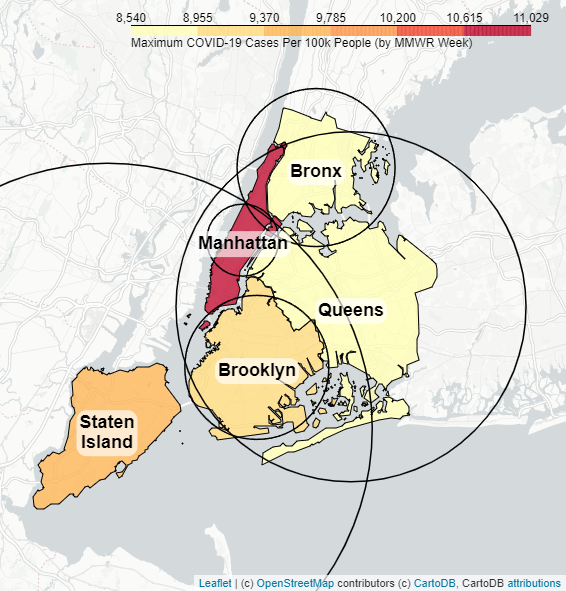
\includegraphics[width=0.48\textwidth]{../plots/cropped-map-avg-trip-distance-at-max-covid-by-pu_borough.png}
    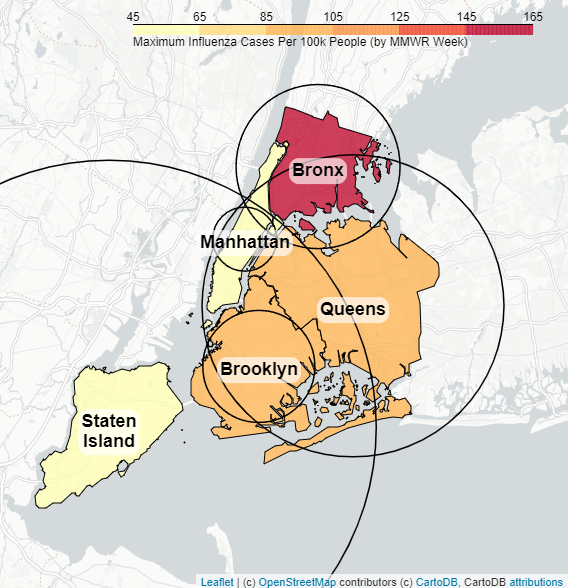
\includegraphics[width=0.48\textwidth]{../plots/cropped-map-avg-trip-distance-at-max-flu-by-pu_borough.png}

    \caption{Map of weekly average trip distance following the maximum COVID-19 (left) and Influenze (right) cases rate over Timeline 2.} % refer to this image as (Figure 1)
    \label{maps}
\end{figure}

\begin{multicols}{2}
    \begin{figure}[H]

        % this ensures your figures are centered where possible
        \centering
    
        % change the scale multiplier to make the figures smaller or larger
        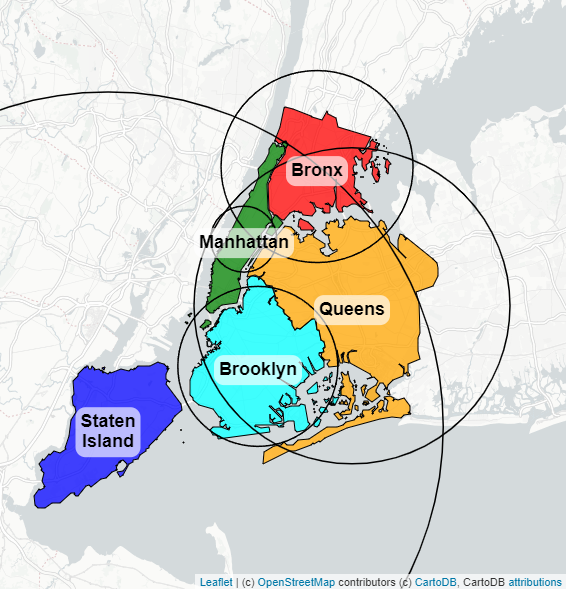
\includegraphics[width=0.5\textwidth]{../plots/cropped-map-avg-trip-distance-overall-pu_borough.png}
    
        \caption{Map of average trip distance overall.} 
        % refer to this image as (Figure 1)
        \label{map:overall}
    \end{figure}
    
    At a first glance, Staten Island experiences the most drastic change in trip distance following instaces of high case rates.
    This contradicts the findings from Figure~\ref{fig:ts}, where the trip radius for Staten Island increased on average.
    On the other hand, this supports the initial expectation that COVID-19 and Influenza prominence will decrease trust in taxi services over long distances
    In general, it appears as though the travel radii per pick-up borough do not change too drastically following an especially high case rate.
    This may be a reflection of the speed at which case data proliferates among the populations of the boroughs,
    since not every individual will be checking last week's case rates.

    The other boroughs do not vary as significantly in trip distance.
    This may be due to their proximity to each other.
    Another contributing factor could be the generally larger populations of these boroughs,
    meaning that a larger proportion of people are unlikely to change their taxi usage based on outside factors.

\end{multicols}

% \begin{figure}[H]

%     % this ensures your figures are centered where possible
%     \centering

%     % change the scale multiplier to make the figures smaller or larger
%     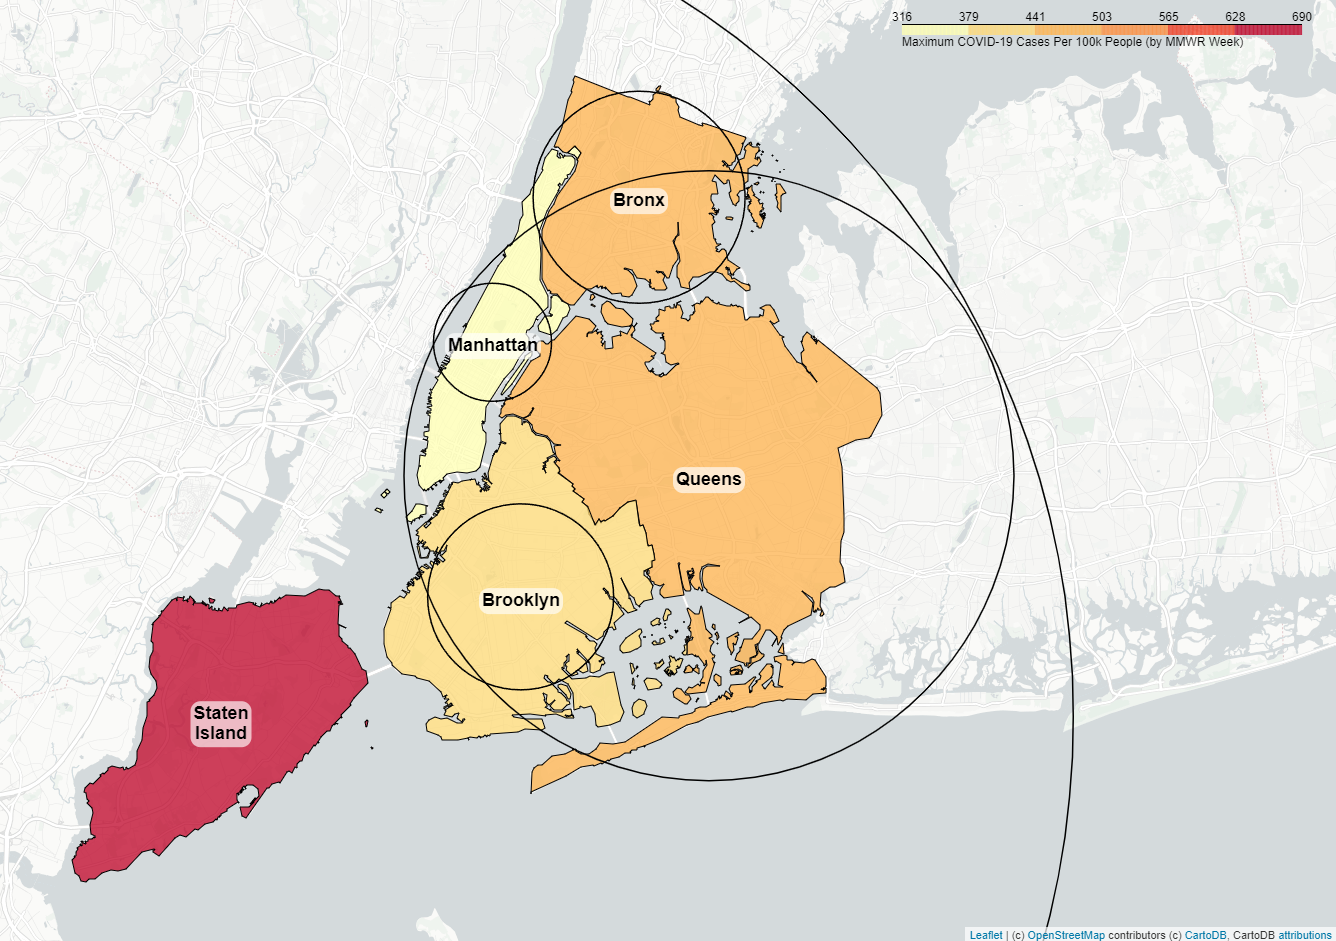
\includegraphics[width=0.45\textwidth]{../plots/map-avg-trip-distance-at-max-covid-by-pu_borough-MODIFIED.png}
%     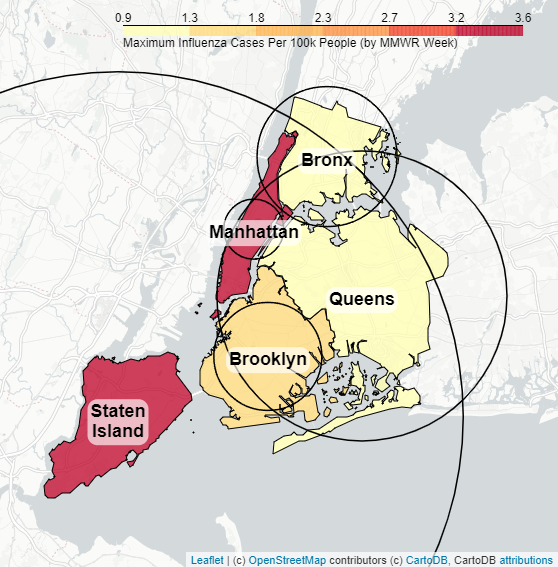
\includegraphics[width=0.45\textwidth]{../plots/map-avg-trip-distance-at-max-flu-by-pu_borough-MODIFIED.png}

%     \caption{Map of weekly average trip distance following the maximum COVID-19 (left) and Influenze (right) cases rate over Timeline 2.} % refer to this image as (Figure 1)
%     \label{maps}
% \end{figure}

% \begin{figure}[H]

%     % this ensures your figures are centered where possible
%     \centering

%     % change the scale multiplier to make the figures smaller or larger
%     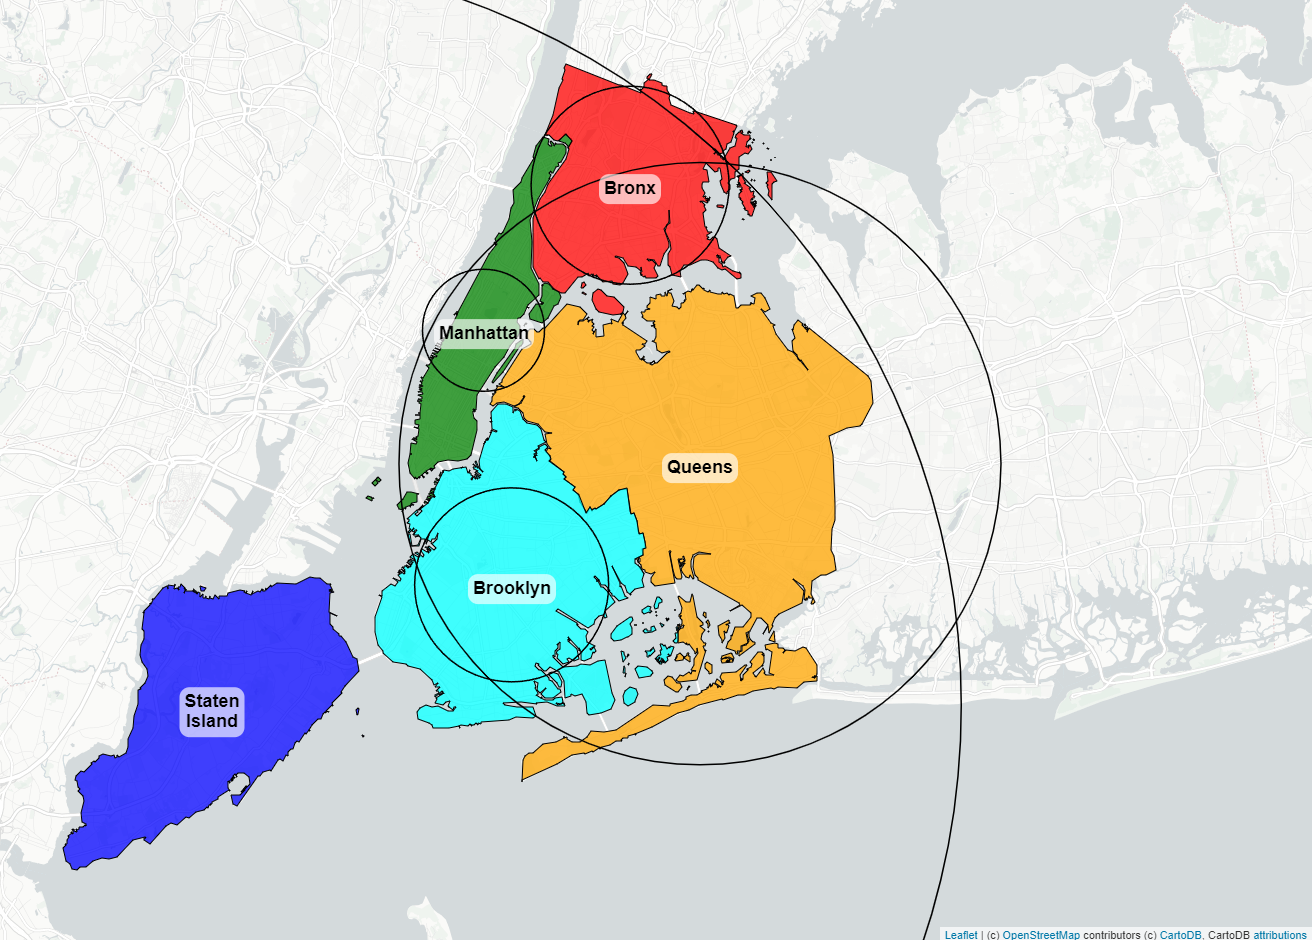
\includegraphics[width=0.5\textwidth]{../plots/map-avg-trip-distance-overall-pu_borough-MODIFIED.png}

%     \caption{Map of average trip distance over Timeline 2.} 
%     % refer to this image as (Figure 1)
%     \label{map:overall}
% \end{figure}

% \end{multicols}


% \begin{figure}[H]

%     % this ensures your figures are centered where possible
%     \centering

%     % change the scale multiplier to make the figures smaller or larger
%     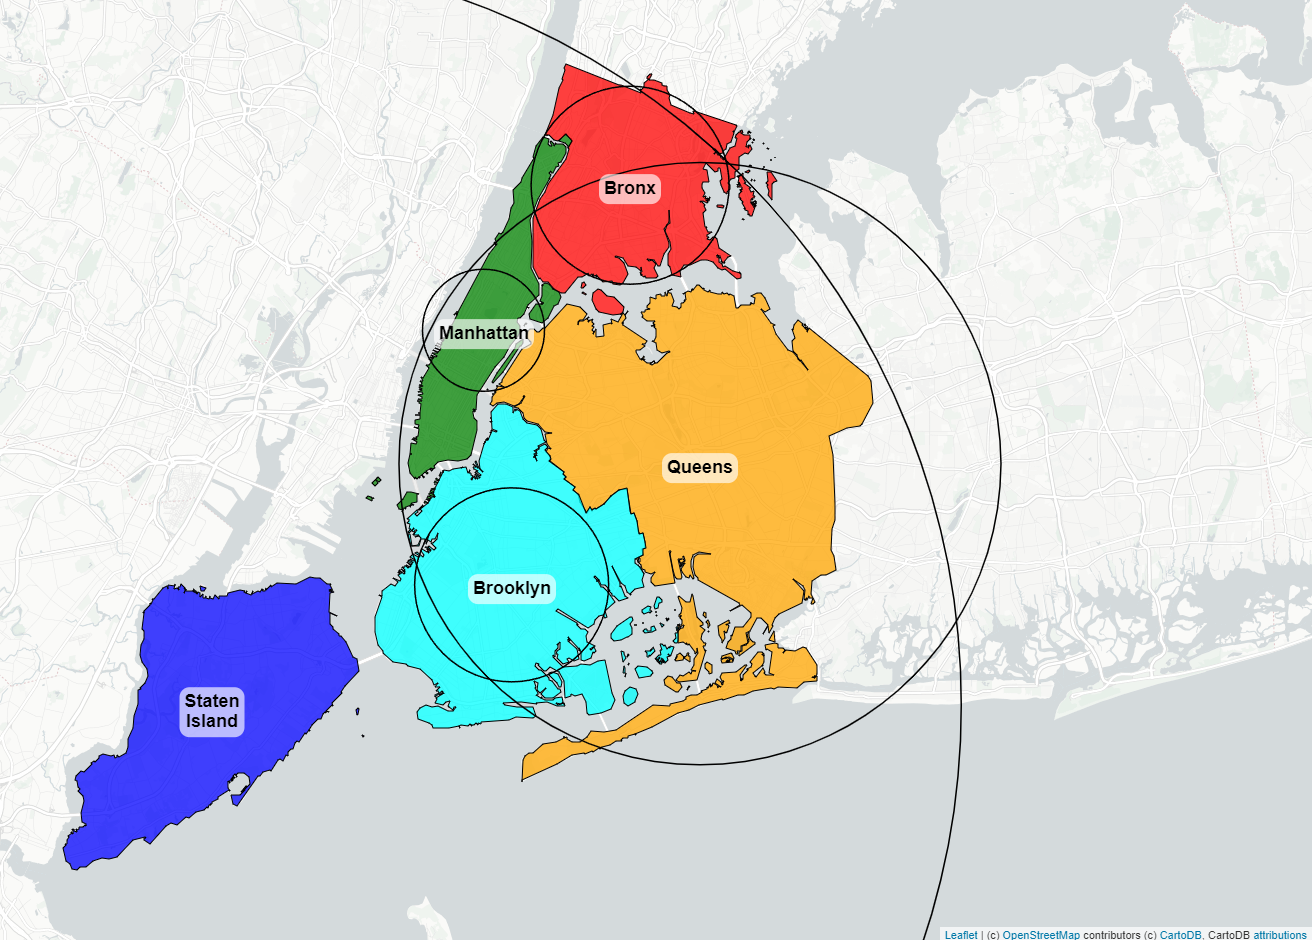
\includegraphics[width=0.45\textwidth]{../plots/map-avg-trip-distance-overall-pu_borough-MODIFIED.png}

%     \caption{Map of average trip distance over Timeline 2.} 
%     % refer to this image as (Figure 1)
%     \label{map:overall}
% \end{figure}

% \pagebreak

% \begin{multicols}{2}

    
    % \begin{figure}[H]
    
    %     % this ensures your figures are centered where possible
    %     \centering
    
    %     % change the scale multiplier to make the figures smaller or larger
    %     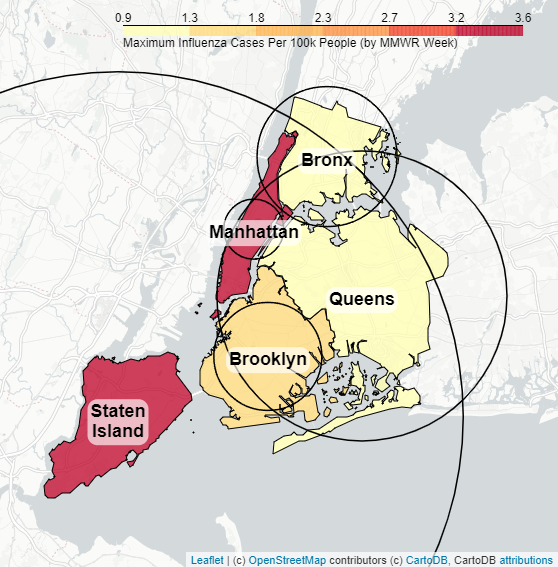
\includegraphics[width=0.45\textwidth]{../plots/map-avg-trip-distance-at-max-flu-by-pu_borough-MODIFIED.png}
    
    %     \caption{Map of weekly average trip distance following the maximum Influenza cases rate over Timeline 2.} % refer to this image as (Figure 1)
    %     \label{map:flu}
    % \end{figure}    
% \end{multicols}

\begin{multicols}{2}
    \textbf{Distributions:} 
It is important to note that the average trip distances
are random variables with a generally unknown distribution.
This means that multiple model candidates may be considered.
In order to select two models to compare and contrast, the distribution of the data
and its properties are investigated.
Trip distances are a continuous metric with a one-sided bound at 0 Miles.

The weekly average trip distances have an overall average of $10.04$ miles, with a variance of $58.75$.
Such a wide variance (where the lower bound of $0$ Miles is only within $2$ standard deviations of the mean) 
suggests that models for trip distances may be more prone to variability with irrelevant predictors.
According to Figure~\ref{fig:hists}, there appear to be multiple peaks in trip distance. 
With fewer bins, there are two discernible peaks, each roughly normally distributed.
With more bins, the peaks are not as easy to discern, nor determine their distributions.
Earlier evidence of positively skewed distribution occurs in Figure~\ref{fig:ts}, 
where there are several bands of average trip distance when grouped by borough.
An argument can be made that Figure~\ref{fig:hists} shows several normally distributed peaks of trip distances.
However, another argument can be made that due to the trip distance being proportional to a measure of duration
with a lower limit at $0$, it can also be approximated with a gamma distribution.

    \begin{figure}[H]
        \centering
        % change the scale multiplier to make the figures smaller or larger
        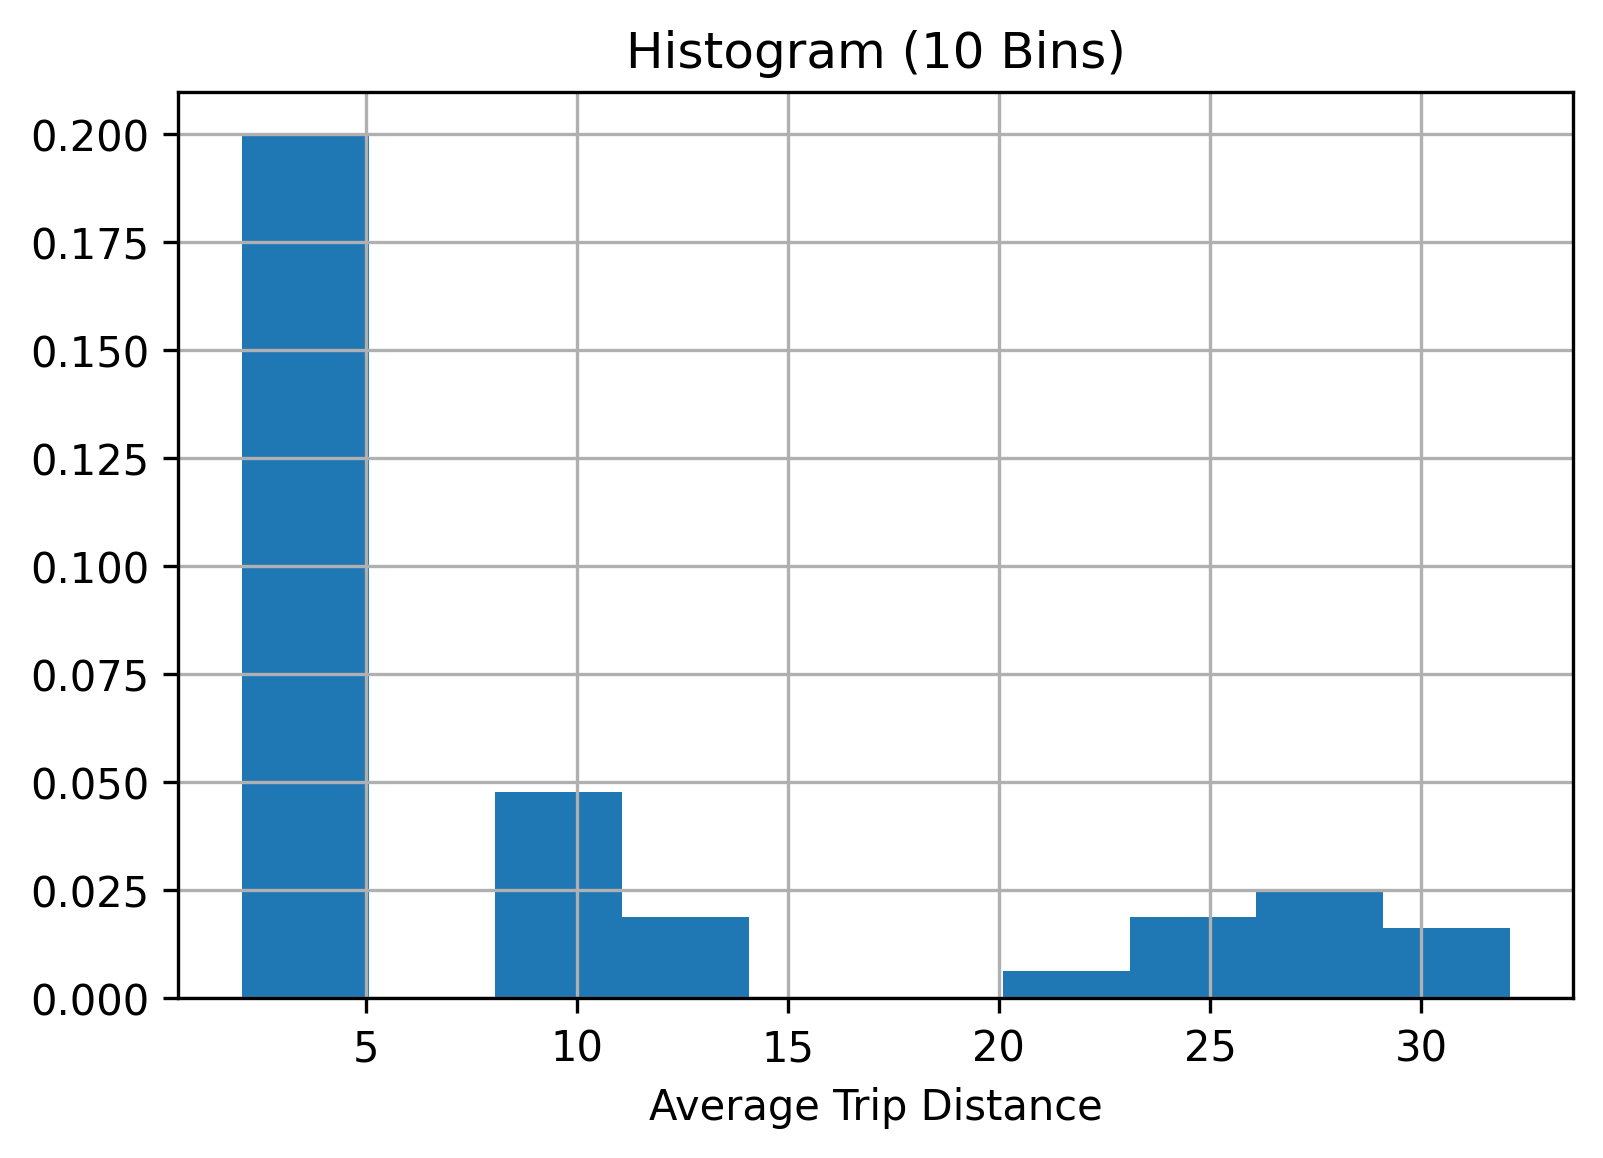
\includegraphics[width=0.5\textwidth]{../plots/histogram-Average Trip Distance-10-bins.png}
        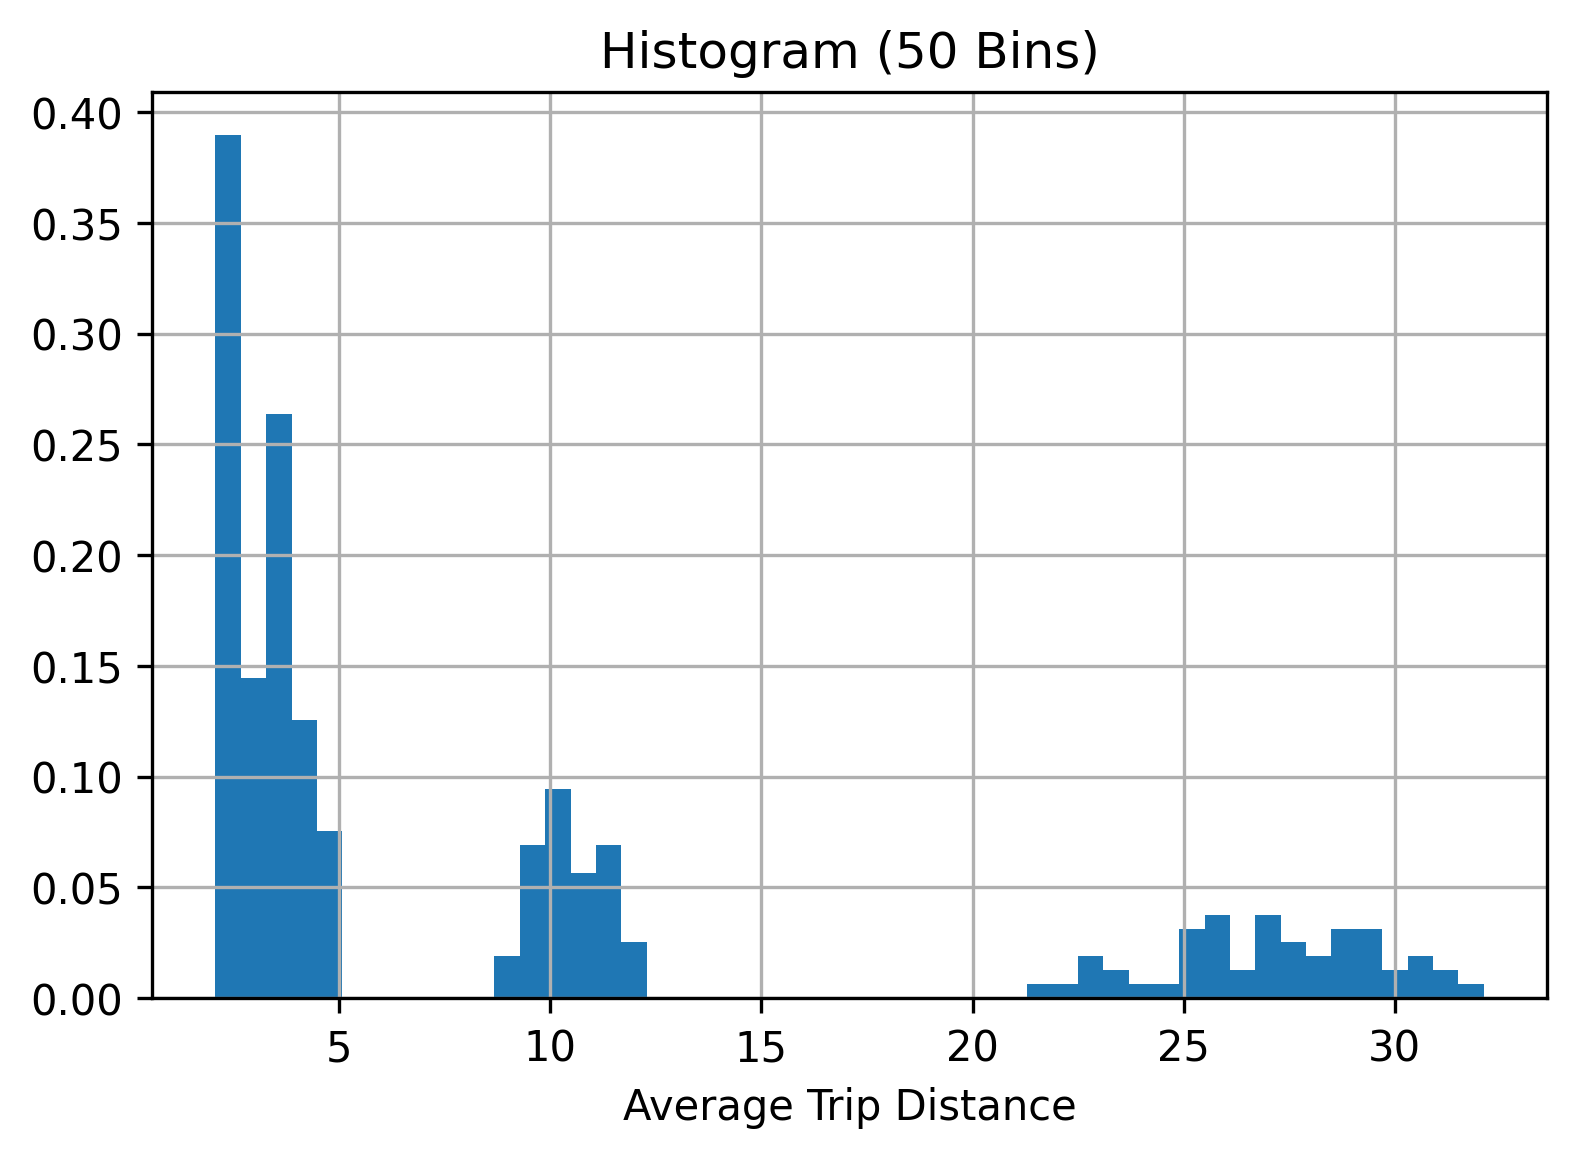
\includegraphics[width=0.5\textwidth]{../plots/histogram-Average Trip Distance-50-bins.png}
        % this ensures your figures are centered where possible
        \caption{Probability density histograms of average trip distance with 10 bins (top) and 50 bins (bottom).} % refer to this image as (Figure 1)
        \label{fig:hists}
    \end{figure}
\end{multicols}
% \textbf{Distributions:} 
% It is important to note that the average trip distances
% are random variables with a generally unknown distribution.
% This means that multiple model candidates may be considered.
% In order to select two models to compare and contrast, the distribution of the data
% and its properties are investigated.
% Trip distances are a continuous metric with a one-sided bound at 0 Miles.


%     \begin{figure}[H]
%         \centering
%         % change the scale multiplier to make the figures smaller or larger
%         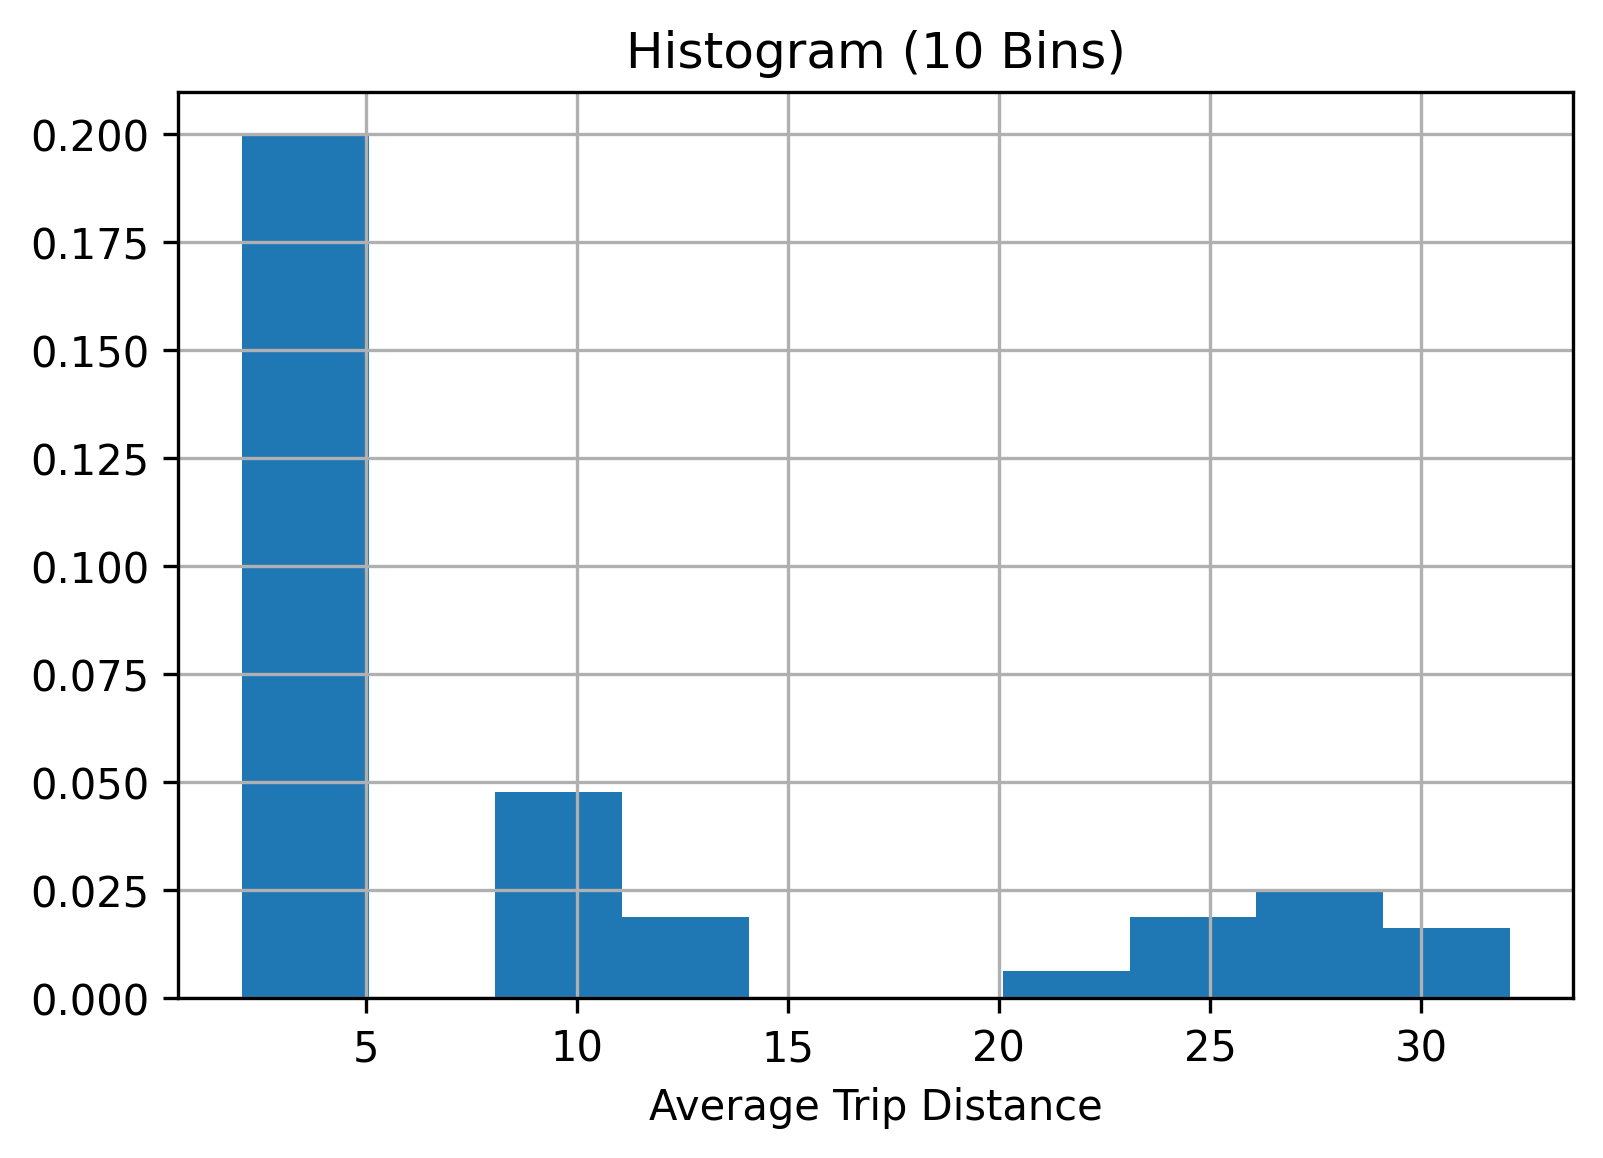
\includegraphics[width=0.5\textwidth]{../plots/histogram-Average Trip Distance-10-bins.png}
%         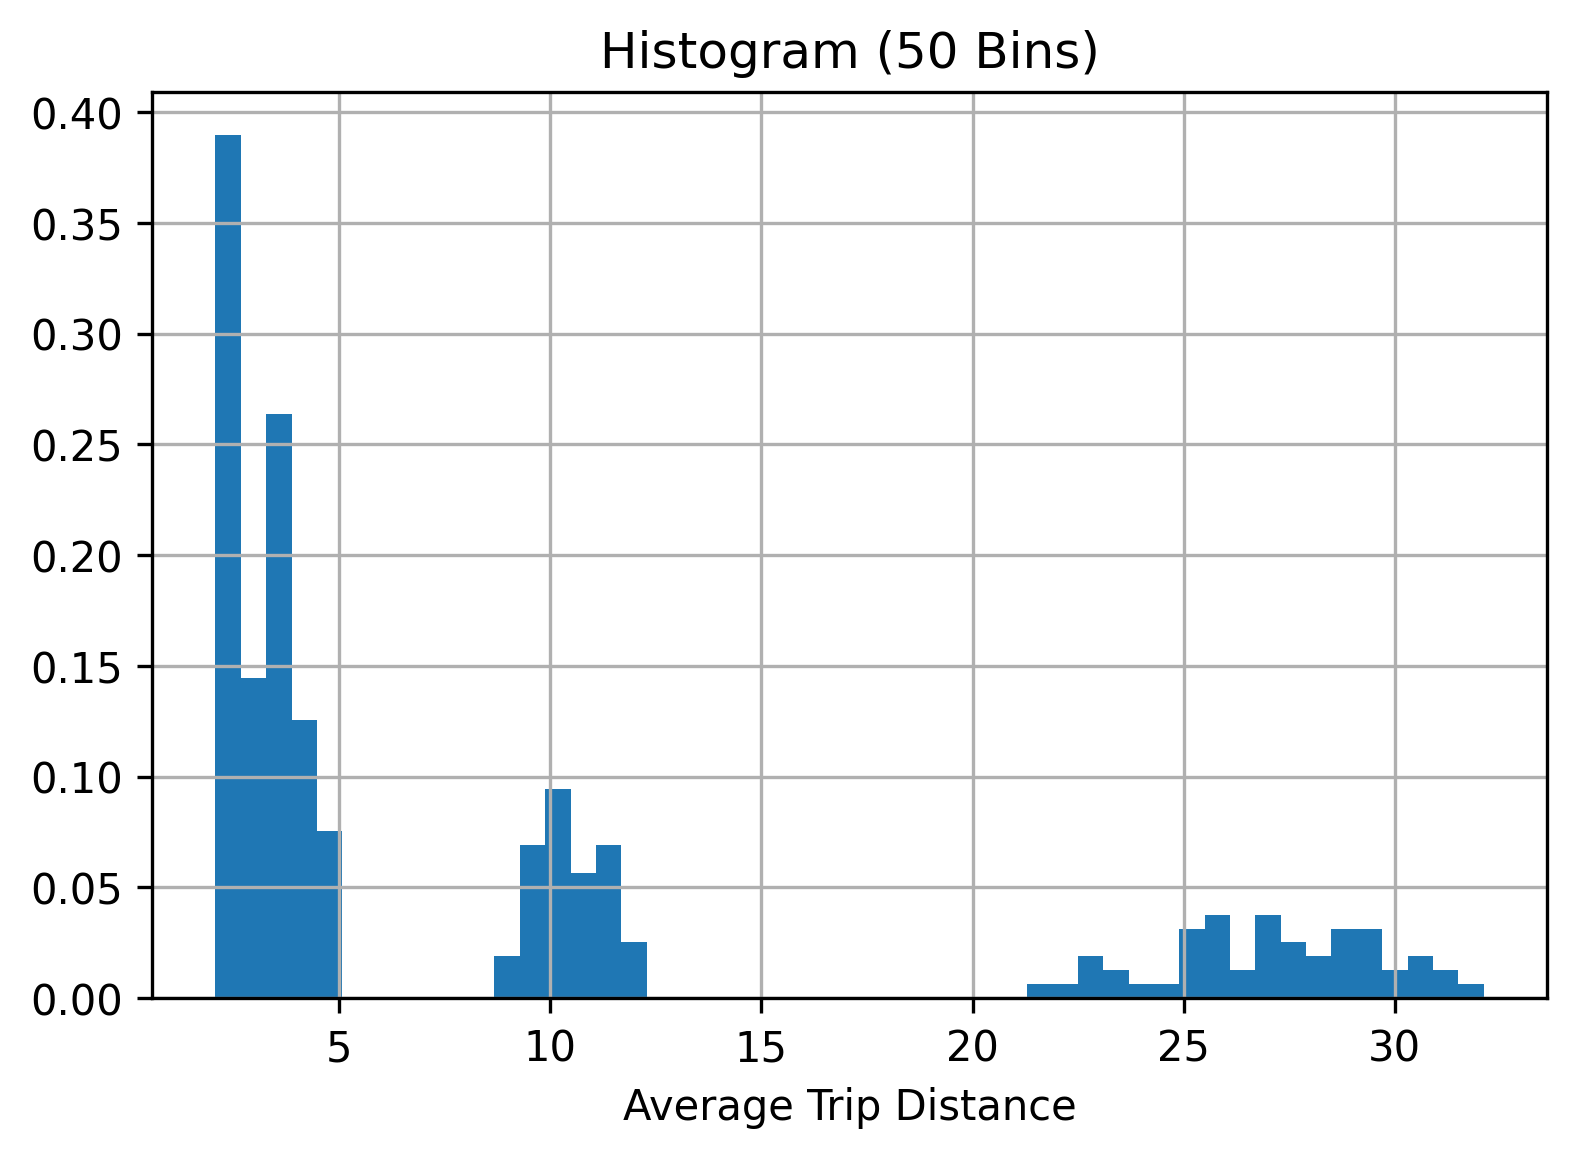
\includegraphics[width=0.5\textwidth]{../plots/histogram-Average Trip Distance-50-bins.png}
%         % this ensures your figures are centered where possible
%         \caption{Probability density histograms of average trip distance with 10 bins (left) and 50 bins (right).} % refer to this image as (Figure 1)
%         \label{fig:hists}
%     \end{figure}

% The weekly average trip distances have an overall average of $10.04$ miles, with a variance of $58.75$.
% Such a wide variance (where the lower bound of $0$ Miles is only within $2$ standard deviations of the mean) 
% suggests that models for trip distances may be more prone to variability with irrelevant predictors.
% According to Figure~\ref{fig:hists}, there appear to be multiple peaks in trip distance. 
% With fewer bins, there are two discernible peaks, each roughly normally distributed.
% With more bins, the peaks are not as easy to discern, nor determine their distributions.
% Earlier evidence of positively skewed distribution occurs in Figure~\ref{fig:ts}, 
% where there are several bands of average trip distance when grouped by borough.
% An argument can be made that Figure~\ref{fig:hists} shows several normally distributed peaks of trip distances.
% However, another argument can be made that due to the trip distance being proportional to a measure of duration
% with a lower limit at $0$, it can also be approximated with a gamma distribution.

\subsubsection{Modelling}

Modelling continuous data is best done with linear models.
Both the pick-up borough and time appear to affect the selected measures of reliance,
meaning that they both need to be considered in the generated models.
This means that for each week's average reliance measure, 
a linear model is generated with the predictors: 
borough,
the preceding week's index in the timeline,
the preceding week's COVID-19 case rate per 100 thousand,
and
the preceding week's Influenza case rate per 100 thousand,
along with interaction between the borough (a non-ordinal categorical)
and each of the viral case rates.

\textbf{Gaussian Linear Model:}
The weekly average trip distance is first modelled using an ordinary least squares (OLS) or Gaussian linear regression,
due to the potential presence of normal distributions per borough.
The generated model displays a negative relationship 
between the viral case rates and trip distances,
due to the parameters being negative ($\beta_{\text{COVID-19}_1} \approx -3 \times 10^{-4}$, and $\beta_{\text{Influenza}_1} \approx -4 \times 10^{-3}$). 
This confirms the theory that increased case rates disincentivise the use of taxis over longer distances.
Other specific OLS parameter values are not mentioned, since this is a less than full rank linear model 
(where there are infinitely many parameter solutions due to the inclusion of a categorical variable).
Instead, the model is analyzed using ANOVA testing and a comparison of fitted and observed data.

\begin{table}[H]
    \centering
    \caption{ANOVA of chosen features in predicting average weekly trip distance}
    \label{tbl:anova1}
    \begin{tabular}{llcccc}
    \hline
                  &                                     & SS                        & DF            & $\mathcal{F}$             & $\mathbb{P}(>\mathcal{F})$        \\ \hline
    \multicolumn{2}{l}{Borough}                         & $2.901 \times 10^{4}$     & $4  $         & $4.438 \times 10^{3}$     & Negligible          \\ \hline
    \multicolumn{2}{l}{Preceding week index}            & $1.136 \times 10^{2}$     & $1  $         & $6.952 \times 10^{1}$     & $7.099 \times 10^{-16 }$          \\ \hline
    \multicolumn{2}{l}{COVID-19 cases}                  & $7.514 \times 10^{0}$     & $1  $         & $4.598 \times 10^{0}$     & $3.249 \times 10^{-2  }$          \\ \hline
                  & Borough Interaction                 & $4.567 \times 10^{0}$     & $4  $         & $6.986 \times 10^{-1}$    & $5.931 \times 10^{-1  }$          \\ \hline
    \multicolumn{2}{l}{Influenza cases}                 & $2.067 \times 10^{1}$     & $1  $         & $1.265 \times 10^{1}$     & $4.115 \times 10^{-4  }$          \\ \hline
                  & Borough Interaction                 & $4.505 \times 10^{2}$     & $4  $         & $6.892 \times 10^{1}$     & $1.313 \times 10^{-46 }$          \\ \hline
    \multicolumn{2}{l}{Residuals}                       & $8.318 \times 10^{2}$     & $509$         &                           &                                   \\ \hline
    \end{tabular}
\end{table}

% \begin{multicols}{2}
    According to Table~\ref{tbl:anova1}, the most significant predictor in the linear model is the borough
    interaction term with Influenza case rates,
    while the least significant is the interaction between COVID-19 cases per 100 thousand and borough.
    At a $95\%$ confidence level, only the COVID-19 interaction terms are considered irrelevant to the model.
    According to Figure~\ref{fig:diag}, the residuals of this model will be heteroskedastic for the data.
    Unfortunately this is a strong indicator that the data does not follow a linear relationship.
    This suggests the need for further investigation into the type of relationship which is present.
    The Gaussian model yields an adjusted $R^2$ of $0.972$, which is generally quite high.
    A measure to consider for comparison to the next is the log-likelihood of the linear regression,
    which is $-865.9$.


\textbf{Gamma Regression:}
Continuous data with bounds that measures duration can often be accurately modelled using a generalized linear model in the gamma family.
Since distance is approximately proportional (if not simply a multiple of) the time duration of each taxi trip,
it may be the case that a gamma regression with the default inverse link is more applicable.
The parameters from this model also supports the theory that trip distance decreases with increased case rates
($\beta_{\text{COVID-19}_2} \approx 6 \times 10^{-6}$, and $\beta_{\text{Influenza}_2} \approx 2 \times 10^{-4}$).
Due to the use of the inverse link function, positive parameter values have an inverse effect on the response.
Again, other specific parameters for the model are not mentioned.
Instead, the relevance of the model can be determined through deviance and the Cox and Snell pseudo $R^2$.
For this data, the model yields a deviance of $4.185$ and a pseudo $R^2$ of $1.000$.
The deviance is very low, which suggests little variance in the model results.
The pseudo $R^2$ is perfect, which indicates that this model is probably overfitting the data.
This model yields a log-likelihood of $-542.2$.

\textbf{Comparing Models:}

According to Figure~\ref{fig:diag}, both the Gaussian and gamma regressions perform well with the given dataset.
While the models are similarly accurate with lower values of trip distance, 
at higher fitted values of trip distance, the ordinary least squares model tends towards a certain trip distance where there is actually a lot of variation.
The gamma model appears to fit results with more homoskedasticity in the data.
This suggests that average trip distances are better modelled using a gamma distribution.

    \begin{figure}[H]
        % change the scale multiplier to make the figures smaller or larger
        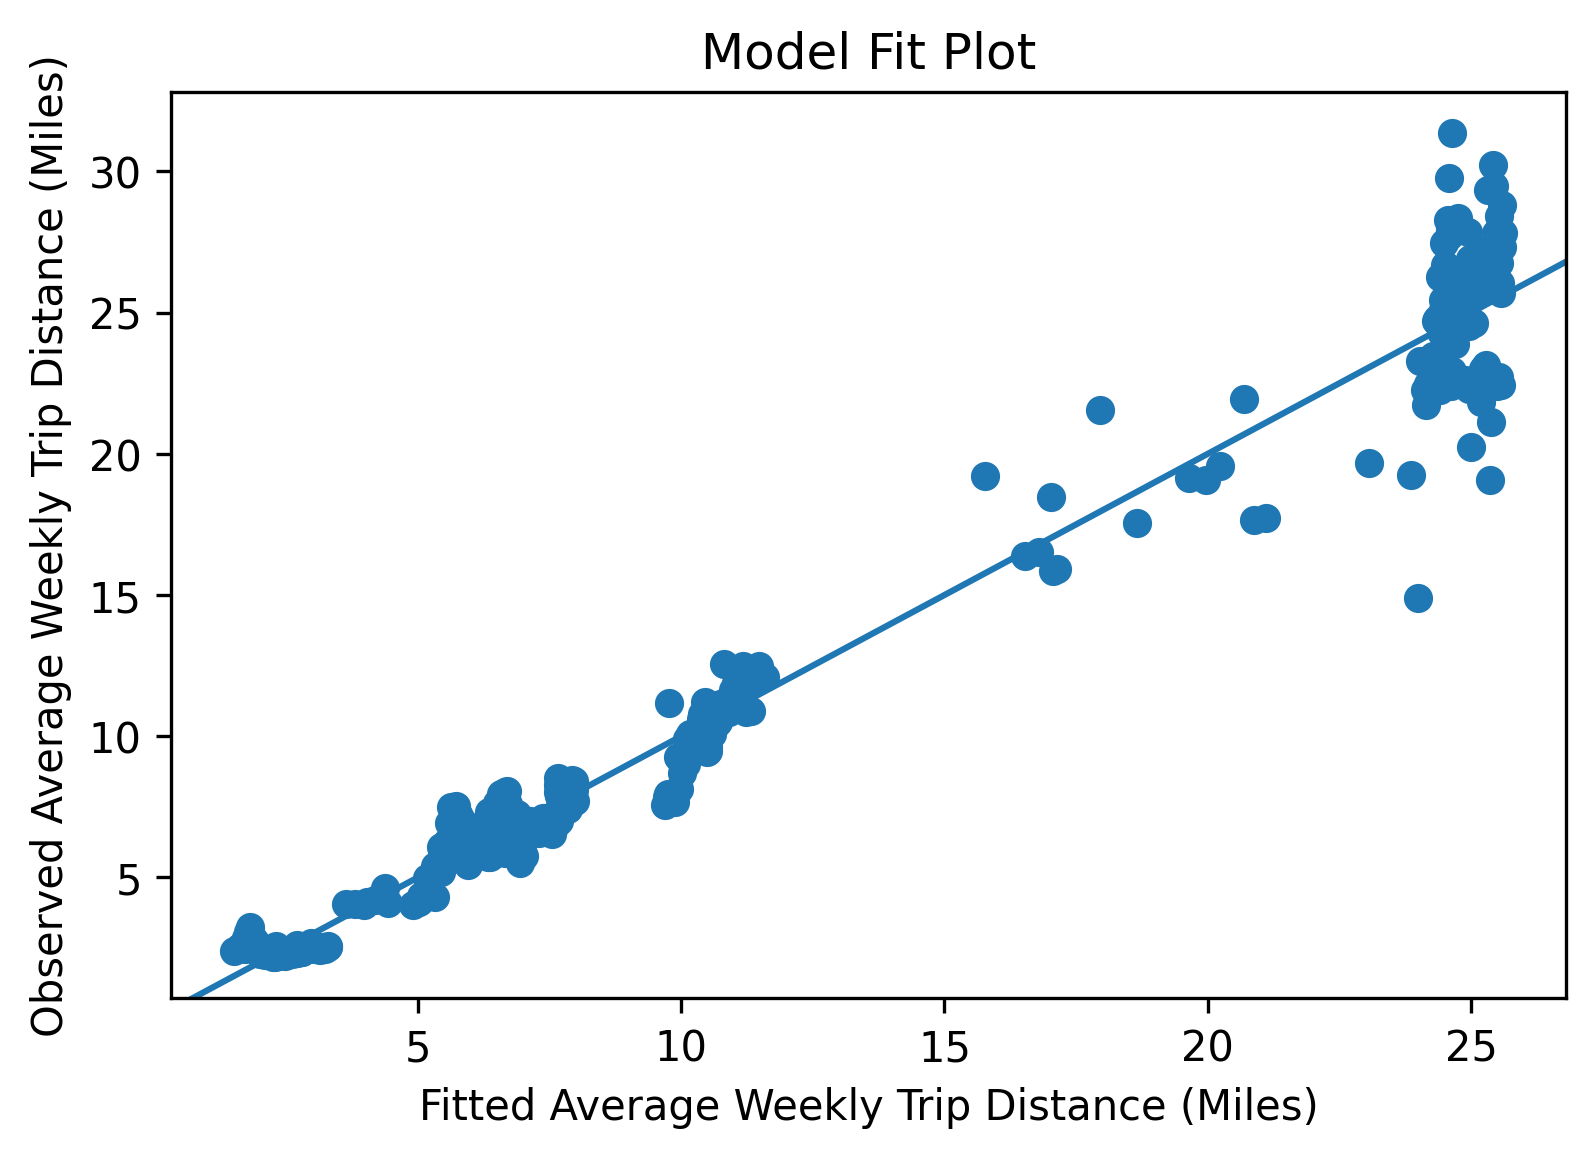
\includegraphics[width=0.49\textwidth]{../plots/diagnostic-ols-Observed Average Weekly Trip Distance (Miles)-vs-Fitted Average Weekly Trip Distance (Miles).png}
        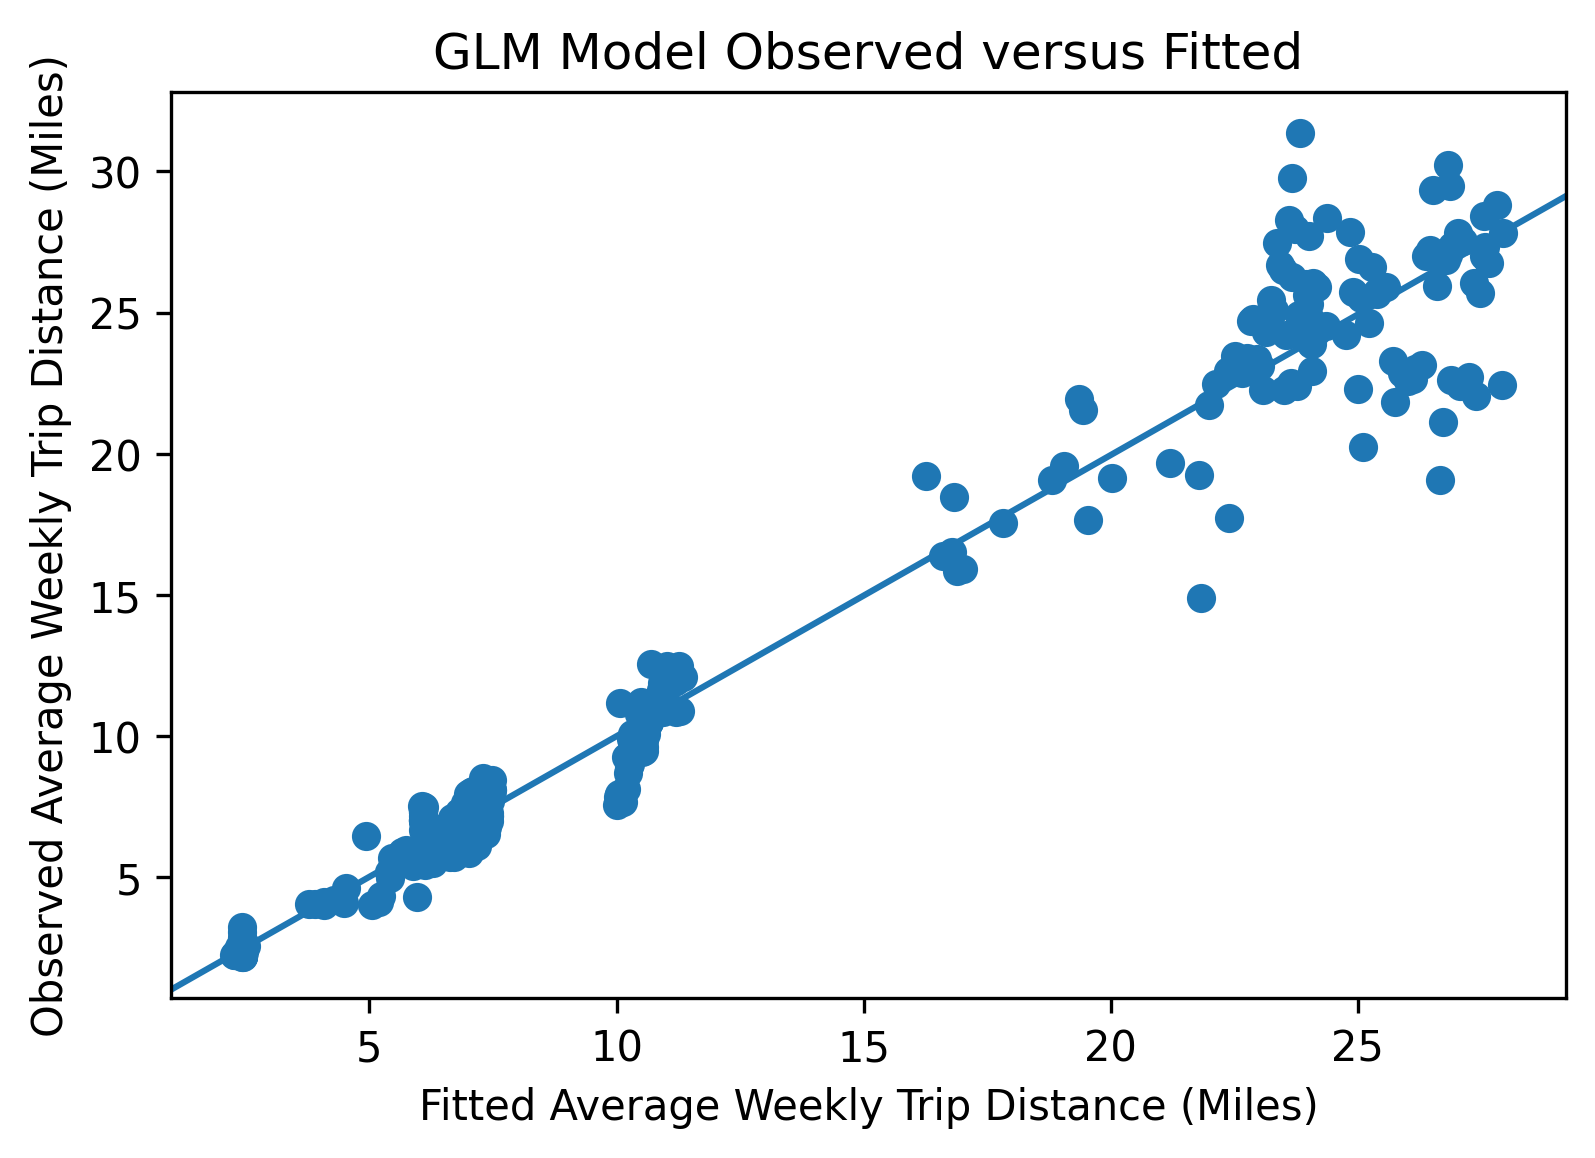
\includegraphics[width=0.49\textwidth]{../plots/diagnostic-glm-Observed Average Weekly Trip Distance (Miles)-vs-Fitted Average Weekly Trip Distance (Miles).png}
        % this ensures your figures are centered where possible
        \centering
        \caption{How observed and fitted values compare for the trip distance Gaussian Linear Regression (left) and gamma Regression (right).} % refer to this image as (Figure 1)
        \label{fig:diag}
    \end{figure}

The models can very easily be compared on their log-likelihoods, since they're both used on the same predictor.
The gamma regression has a log-likelihood of $-542.2$, whereas the Gaussian (OLS) regression has a log-likelihood of $-865.8$.
Since the gamma regression has a higher log-likelihood, the probability of its parameters being more correct
is higher. This suggests that the trip distance data is indeed better represented with a gamma regression model.

% \end{multicols}

% \begin{multicols}{2}
%     \textbf{Weekly Average Passenger Count:}
% The passenger count in each trip is a discrete metric
% likely described by a Poisson distribution with a rate parameter $\lambda$, 
% while the average passenger count/rate per trip per week is a rate value on a continuous scale.
% If the data was aggregated per trip, then it could be modelled with a simple Poisson regression.
% However, since the estimated rate of a Poisson random variable is complicated to model,
% it is preferrable to model the total count of passengers in each trip in a week
% using a Poisson regression with an offset equal to the logarithm of the number of trips \cite{poisson}.
% This is derived using the log link function in a generalized linear model attempting to model passenger rate:

% \begin{align*}
%     \log \left[\frac{\text{Passenger Count}}{\text{Number of Trips}}\right] &= X\hat{\beta} \\
%     \implies \log \left[\text{Passenger Count}\right] &= X\hat{\beta} \\
%     &+ \log \left[\text{Number of Trips}\right]
% \end{align*}

% \end{multicols}
% \pagebreak
% \begin{multicols}{2}

% %     \begin{figure}[H]
% %         % change the scale multiplier to make the figures smaller or larger
% %         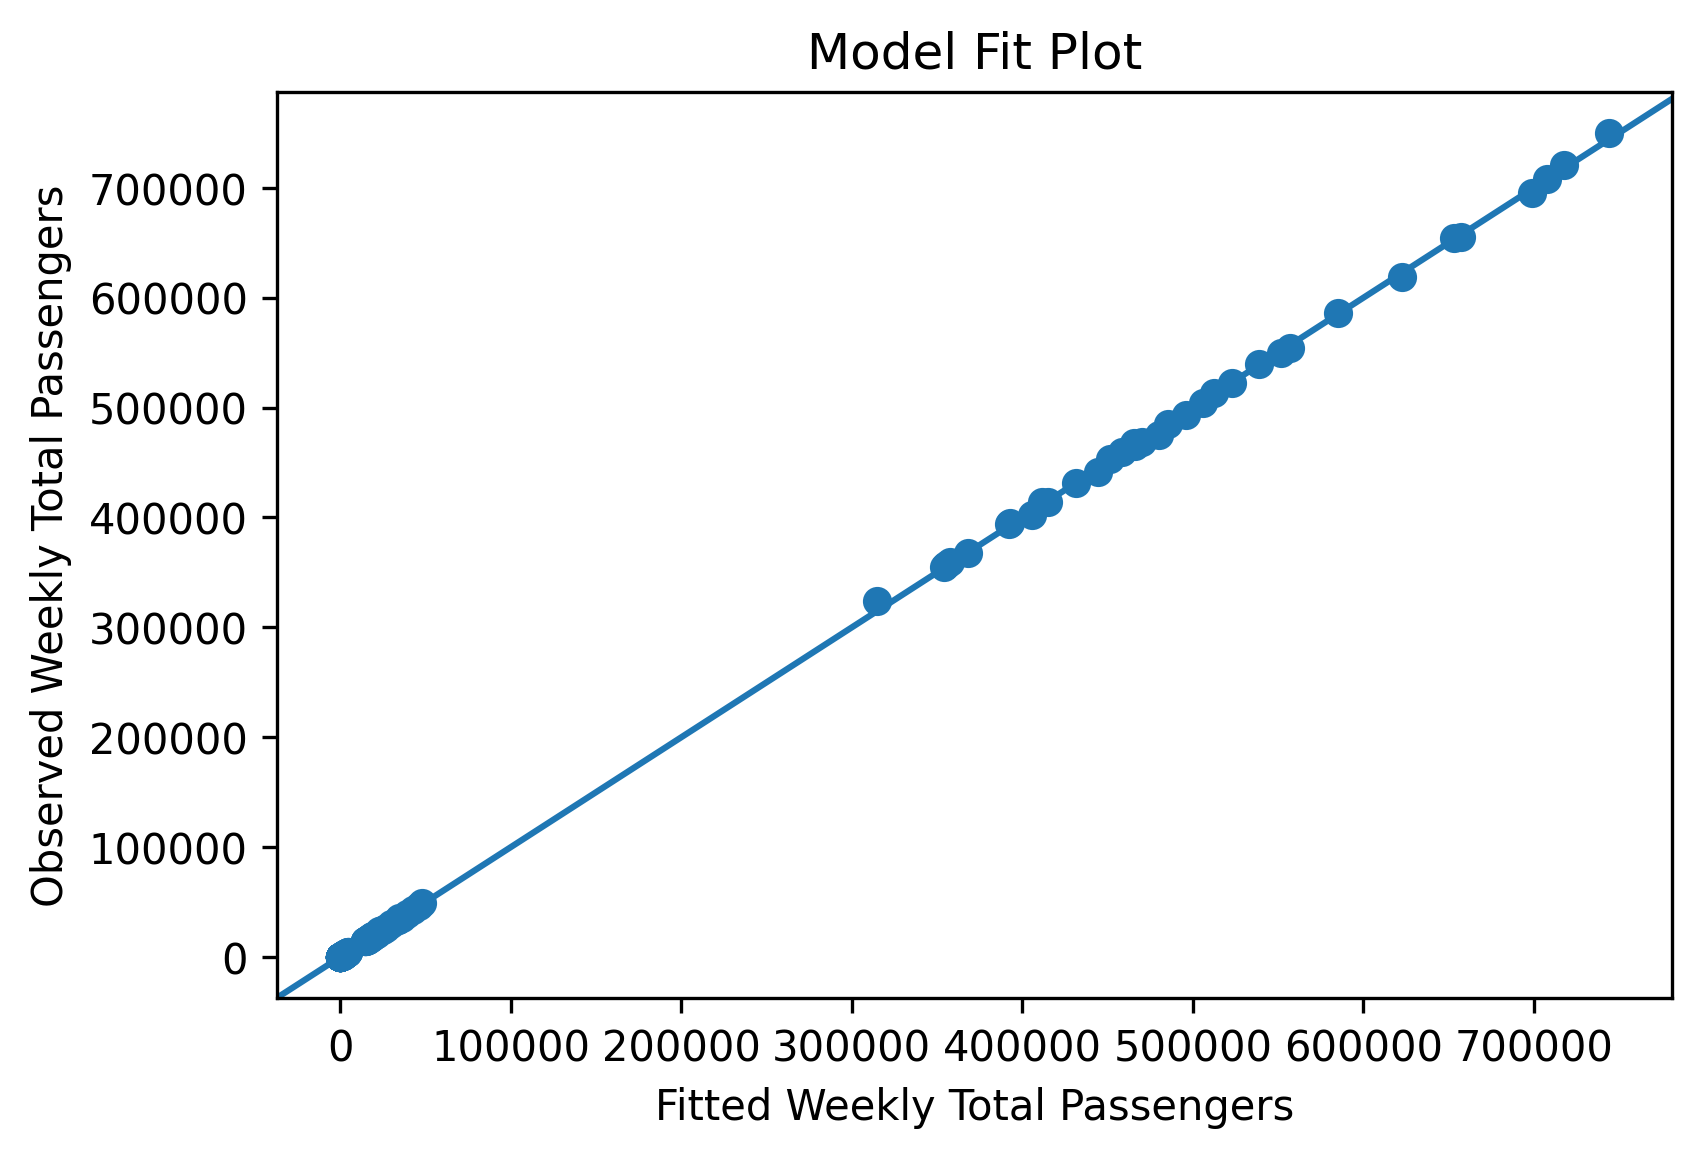
\includegraphics[width=0.51\textwidth]{../plots/diagnostic-Observed Weekly Total Passengers-vs-Fitted Weekly Total Passengers.png}
% %         % this ensures your figures are centered where possible
% %         \centering
% %         \caption{How observed and fitted values compare for total passenger counts in the Poisson regression.} % refer to this image as (Figure 1)
% %         \label{fig:glm}
% %     \end{figure}

% %     Again, there is no single solution for the parameters of this model due to the input data containing a categorical predictor.
% % Instead the resulting $p$-values for each parameters can be analyzed to see if any relationships are irrelevant to modelling passenger counts.
% % Specifically high is the $p$-value for the $z$ statistic of Influenza total cases with a value of $p = 0.415$, 
% % suggesting that with even a $95\%$ confidence level, 
% % Influenza has little correlation to reliance on taxis.
% % According to Figure~\ref{fig:glm}, this model appears to strictly conform to the observations given.
% % This might unfortunately also be an indicator of overfitting in the data,
% % which would require further data to be collected and checked against to confirm.

% \end{multicols}



% \begin{enumerate} 
%     \item Example for enumerated points
%     % use \item to create more points
% \end{enumerate}

% \begin{itemize} 
%     \item Example for dot points
%     \item[*] You can change dot points to any symbols by putting [SYMBOL].
%     \item[$\times$] Here's a fun example.
% \end{itemize} 
% \lipsum[4-5]
% Example code for figures:
% % the [h] ensures your figure is inline at the location and not displayed on some other page
% \begin{figure}[h]
%     % change the scale multiplier to make the figures smaller or larger
%     \includegraphics[width=0.35\textwidth]{example-image-a}
%     % this ensures your figures are centered where possible
%     \centering
%     \caption{Some caption} % refer to this image as (Figure 1)
% \end{figure}
% \lipsum[1-2]

% Example of a maths equation:
% \begin{equation}
%     Y = X\beta + \epsilon
% \end{equation}

% Example of an aligned equation (\& denotes the symbol to align):
% \begin{align*}
%     E[\mathbf{y}] &= X\beta + E[0] \\
%                   &= X\beta
% \end{align*}

% Example of an in-line equation $\epsilon \sim N(0, 1)$ \\

\section{Conclusions}

In conclusion, there is merit to the thinking that increased case rates of viruses 
have an effect on the reliance on taxis at different distances.
According to the linear models generated, 
both COVID-19 and Influenza have a small, but relevant relationship with the average taxi trip's distance.
These relationships can be shown either with an ordinary least squares linear regression,
or with a gamma regresion, with the latter yielding a higher $R^2$.
However, there is the risk that the latter is overfitting the data,
which may be the case due to the relatively small ($< 1000$ points) sample size.
It is important to note that no causal relationships were proven or investigated in this report,
and thus the generated models cannot be relied on as anything more than indicators
of underlying correlations. In the same vein, 
while the models can be used to predict future reliance measures of yellow taxis,
they should by no means be the sole models used. 
Instead they are best suited for use in conjunction with several others.



\section{Further Research}
There are several paths for further research based on this report.
First, consider other datasets which merit inclusion
in this analysis, such as other virus case rates, or other forms of transport.
With more data to analyze, a clearer picture of the true relationships between infectious disease and preceived need for transport services.
As mentioned in the paper, the TLC data is aggregated by pick-up location.
    The same analysis should also be performed on aggregation by drop-off location.
    There may be value in comparing and contrasting the resulting models with this different grouping.
Finally, specifically select a subset of specific locations where trips going to/from are likely work-related. 
This would provide a window into measuring the shift to working from home caused by viruses.


\clearpage

% BEGIN REFERENCES SECTION
\printbibliography

\end{document}